\chapter{Experimental results and discussion}
\label{chap:experimental-results}

This chapter presents the experimental results from the validation campaign for the LINKU stereo vision system. The analysis is organized to progressively evaluate the limitations of conventional photogrammetric approaches, the performance of the proposed geometry-driven reconstruction methodology, and the potential role of AI-assisted techniques for future system evolution.
\\\\
The experimental results are analyzed with respect to the optical constraints identified in Chapter \ref{chap:theoretical-optical-analyses}, the geometry-driven and AI-assisted reconstruction methodologies introduced in Chapter \ref{chap:experimental-processing-approaches}, and the validation platform and orbital-like observation environment described in Chapter \ref{chap:experimental-setup-hardware-config}.
\\\\
Particular emphasis is placed on assessing the system's ability to detect, localize, and reconstruct thin tether-like structures under low-texture and high-contrast observation conditions. These conditions are representative of the visual challenges expected during orbital tether deployment and post-deployment characterization phases.
\\\\
The chapter first examines the performance of conventional photogrammetry under space-emulated conditions to establish a reference baseline. The results are then compared with those obtained using the proposed geometry-driven reconstruction framework, followed by an assessment of exploratory AI-assisted reconstruction approaches. Together, these analyses provide a comprehensive evaluation of the strengths, limitations, and operational suitability of the proposed stereo vision system.

\section{Validation objectives and experimental datasets}
\label{sec:validation-objectives-experimental-datasets}

The experimental campaign was designed to evaluate the feasibility of reconstructing tether geometry under conditions representative of orbital observation.
\\\\
The validation process focused on three principal objectives:
\begin{enumerate}
    \item Assessing the limitations of conventional feature-based photogrammetry.
    \item Validating the geometry-driven reconstruction methodology proposed in Chapter \ref{chap:experimental-processing-approaches}.
    \item Investigating the potential applicability of AI-assisted reconstruction techniques.
\end{enumerate}

Two experimental datasets were employed throughout the validation campaign. The first consisted of a volumetric reference object (Figure \ref{fig:figure5.3}), while the second utilized a 1 mm tether proxy representative of the geometry considered in the LINKU mission concept (Figure \ref{fig:figure5.5}). These datasets were used to evaluate both conventional photogrammetric techniques and the geometry-driven reconstruction methodology under controlled laboratory conditions.
\\\\
The tether reconstruction experiments were evaluated under two representative geometric configurations.

\begin{itemize}
    \item Scenario A corresponds to a predominantly planar configuration in which the tether remained approximately parallel to the image plane, resulting in limited depth variation.
    \item Scenario B introduces significant out-of-plane deformation and depth variation, creating a more challenging reconstruction problem that better represents realistic deployment dynamics.
\end{itemize}

All datasets were acquired using the calibrated stereo imaging platform described in Chapter 5 and processed using identical calibration parameters to ensure consistency throughout the experimental campaign.

\section{Evaluation of conventional photogrammetry}
\label{sec:evaluation-conventional-photogrammetry}

Before developing the geometry-driven reconstruction methodology, a series of experiments were conducted to evaluate the suitability of conventional photogrammetric techniques for tether observation under orbital-like conditions. These tests were intended to establish a reference baseline and identify the principal failure modes associated with feature-based stereo reconstruction in low-texture environments.
\\\\
The evaluation focused on the experimental targets introduced in Chapter \ref{chap:experimental-setup-hardware-config}. The volumetric reference object (Figure \ref{fig:figure5.3}) was used to assess the behavior of conventional dense stereo reconstruction under reduced-texture conditions, while the tether proxy (Figure \ref{fig:figure5.5}) was employed to evaluate the applicability of commercial Structure-from-Motion (SfM) techniques to thin tether-like geometries.
\\\\
The results demonstrate that although conventional photogrammetry performs adequately when sufficient texture is available, its performance rapidly degrades as environmental features disappear. These observations provide direct experimental evidence supporting the optical limitations discussed in Chapter \ref{chap:theoretical-optical-analyses} and motivate the development of the geometry-driven reconstruction strategy presented in Chapter \ref{chap:experimental-processing-approaches}.

\subsection{Volumetric object reconstruction under low-texture conditions}
\label{sub:volumetric-object-reconstruction}

A preliminary validation experiment was performed using the volumetric reference object introduced in Figure \ref{fig:figure5.3}. The objective was to evaluate the behavior of conventional dense stereo reconstruction when operating inside the low-texture environment provided by the dark enclosure described in Section \ref{subsub:Dark-enclosure}.

The reconstruction was generated using a standard dense stereo workflow based on disparity estimation and three-dimensional point triangulation. Although the object remained clearly visible in the stereo imagery, the absence of surrounding visual features significantly degraded the reliability of the matching process.

Figure \ref{fig:figure6.1} illustrates the origin of the reconstruction failure. The disparity map in Figure \ref{fig:figure6.1}(a) correctly identifies the volumetric target through its high disparity values, which correspond to the shortest camera-to-object distances. However, non-physical disparity responses also appear throughout regions that should correspond to empty background space. These erroneous matches propagate into the reconstructed coordinate maps shown in Figures \ref{fig:figure6.1}(b) and \ref{fig:figure6.1}(c), where spatially inconsistent points emerge outside the physical boundaries of the object.
\newpage
\clearpage

\begin{figure}[!ht]
    \centering
    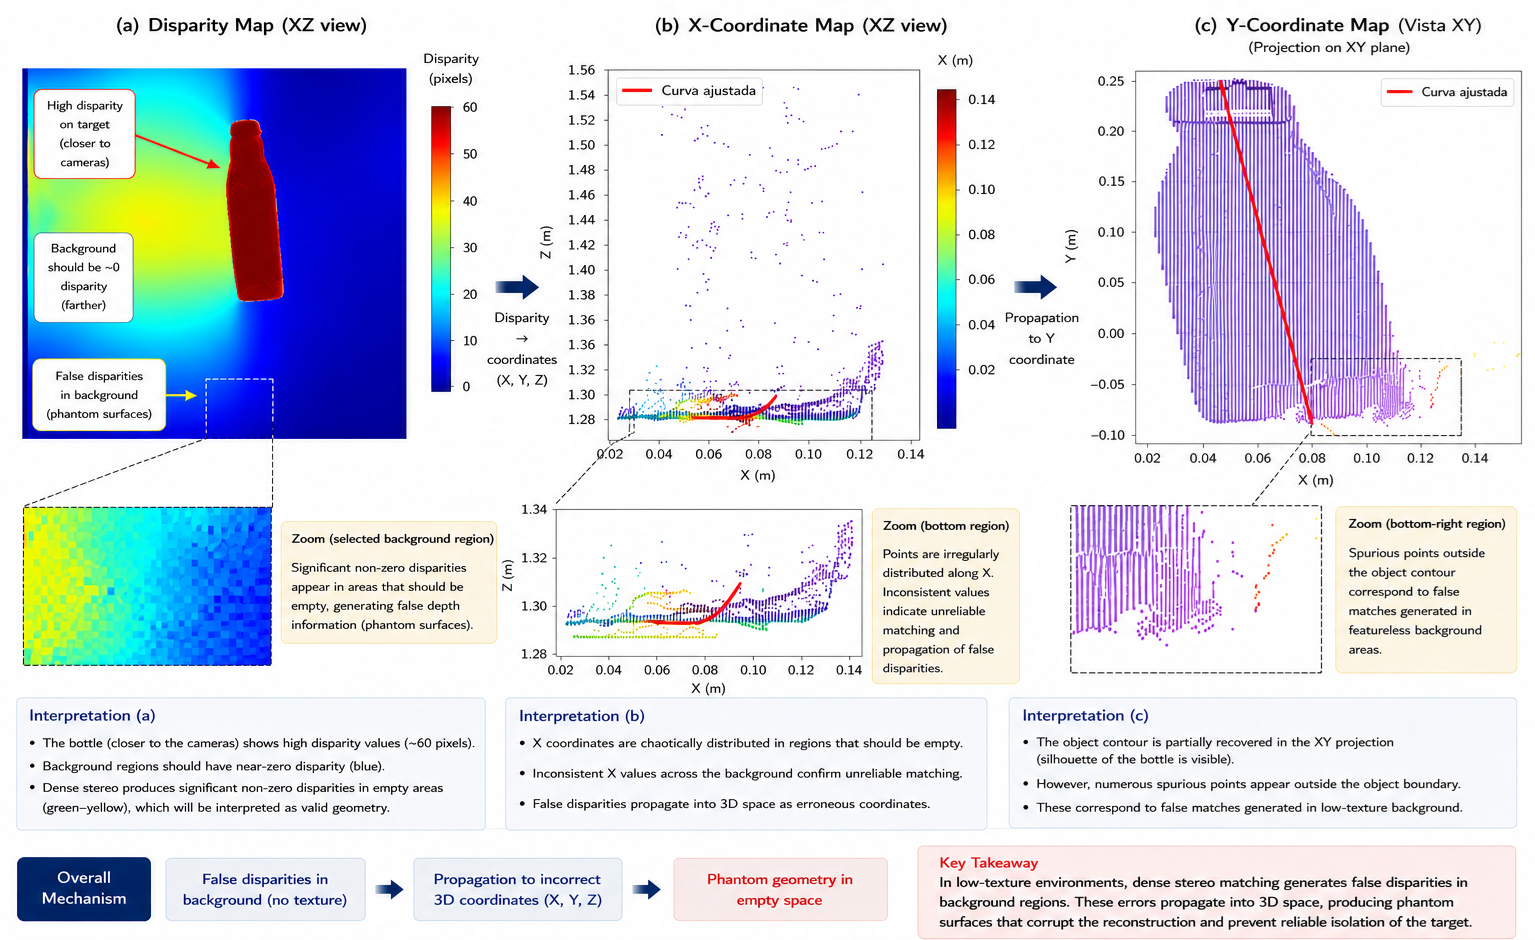
\includegraphics[width=\textwidth]{Images/Figure 6.1.png}
    \caption[Failure mechanism of conventional dense stereo reconstruction under Low-texture conditions.]{Failure mechanism of conventional dense stereo reconstruction under Low-texture conditions.}
    \label{fig:figure6.1}
\end{figure}

The resulting disparity artifacts generate phantom geometric structures that do not correspond to any real surface within the scene. Although portions of the target geometry remain identifiable, the presence of false correspondences introduces substantial ambiguity into the three-dimensional reconstruction process.
\\\\
The consequences of these errors are presented in Figure \ref{fig:figure6.2}. The raw point cloud contains numerous outliers and phantom surfaces due to incorrect disparity estimates in low-texture regions. %To isolate the volumetric target, extensive manual filtering was required to remove spurious points and background artifacts. Only after this intervention could a partial representation of the object be recovered and approximated through geometric fitting.
%\newpage
%\clearpage

\begin{figure}[!ht]
    \centering
    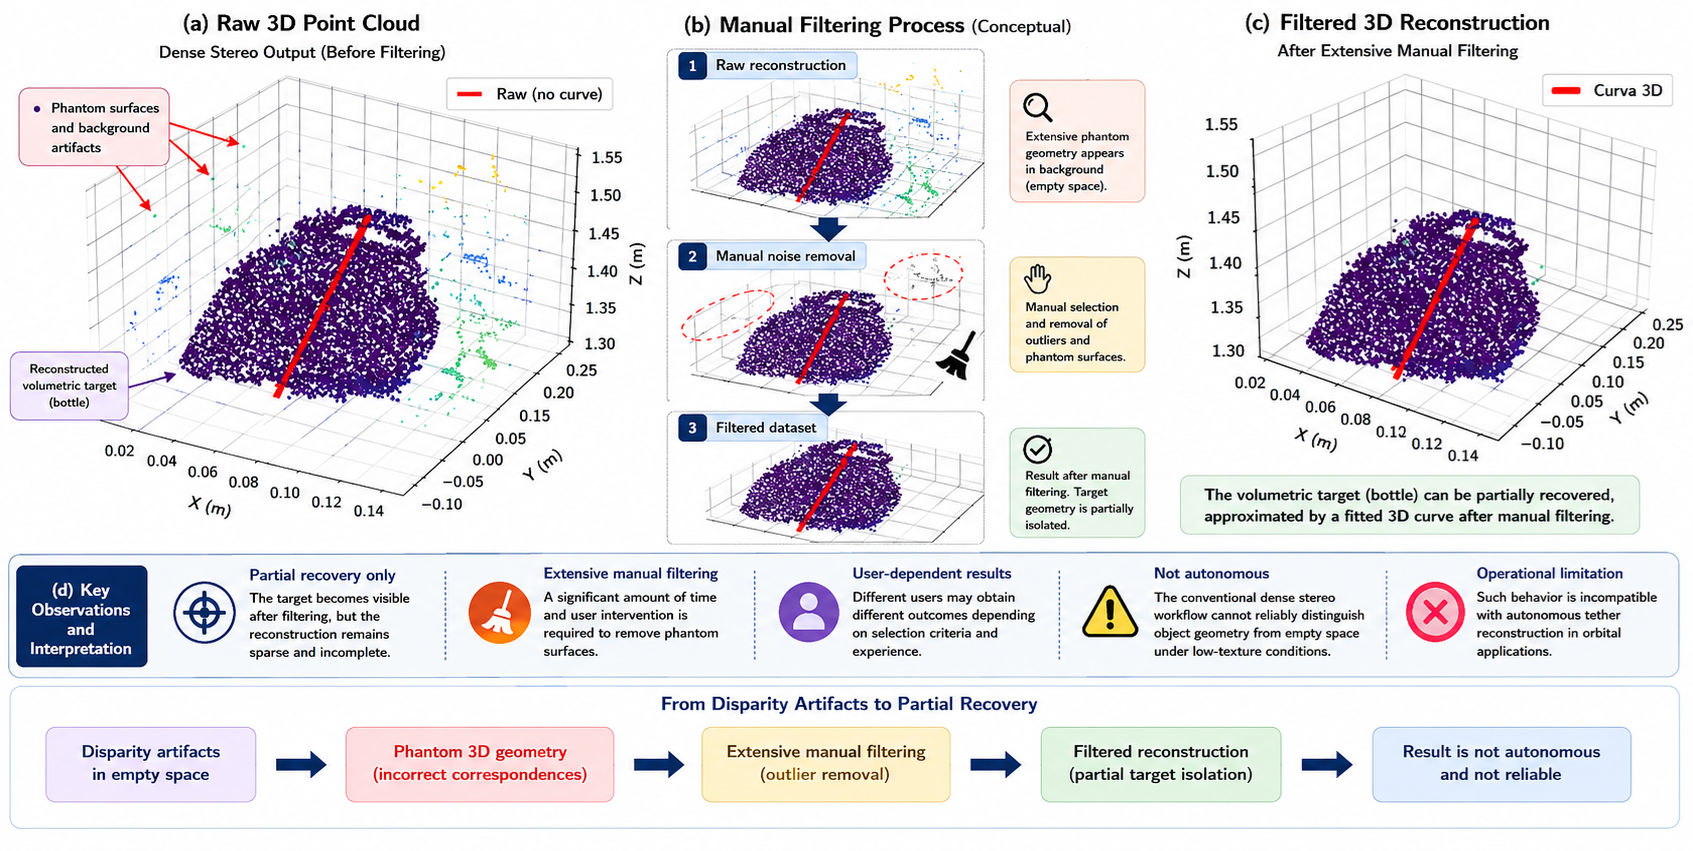
\includegraphics[width=\textwidth]{Images/Figure 6.2.png}
    \caption[Filtered three-dimensional reconstruction after manual removal of disparity artifacts.]{Filtered three-dimensional reconstruction after manual removal of disparity artifacts. The figure shows consequences of disparity estimation error on the final 3D reconstruction, which is the manual filtering for target isolation.}
    \label{fig:figure6.2}
\end{figure}

These results demonstrate that conventional dense stereo reconstruction remains strongly dependent on environmental texture and visual context. While the target object can still be partially recovered, the reconstruction process requires significant user intervention and is therefore not autonomous. Such behavior would be incompatible with operational tether-monitoring scenarios, where robust, automatic reconstruction must be achieved under similarly low-texture orbital observation conditions.

\subsection{Tether reconstruction against textured and texturedless background conditions}
\label{sub:tether-reconstruction-failure}

To further investigate the limitations of conventional photogrammetric reconstruction, the tether proxy introduced in Figure \ref{fig:figure5.5} was processed using a commercial Structure-from-Motion (SfM) workflow. Unlike the volumetric reconstruction experiment presented in Section \ref{sub:volumetric-object-reconstruction}, the objective of this test was to evaluate whether a thin tether-like structure could be reconstructed under conditions representative of the LINKU mission scenario.
\\\\
Figure \ref{fig:figure6.3} presents the reconstruction obtained when the tether was observed within a textured environment containing multiple visual features, including floor patterns, object edges, and surrounding structures. Under these conditions, the SfM pipeline successfully detected image features, established reliable correspondences, aligned the camera poses, and generated a valid three-dimensional reconstruction. However, inspection of the reconstructed scene reveals that the majority of the recovered geometry originates from the surrounding environment rather than from the tether itself. The reconstruction process therefore remains strongly dependent on environmental texture.

\begin{figure}[!ht]
    \centering
    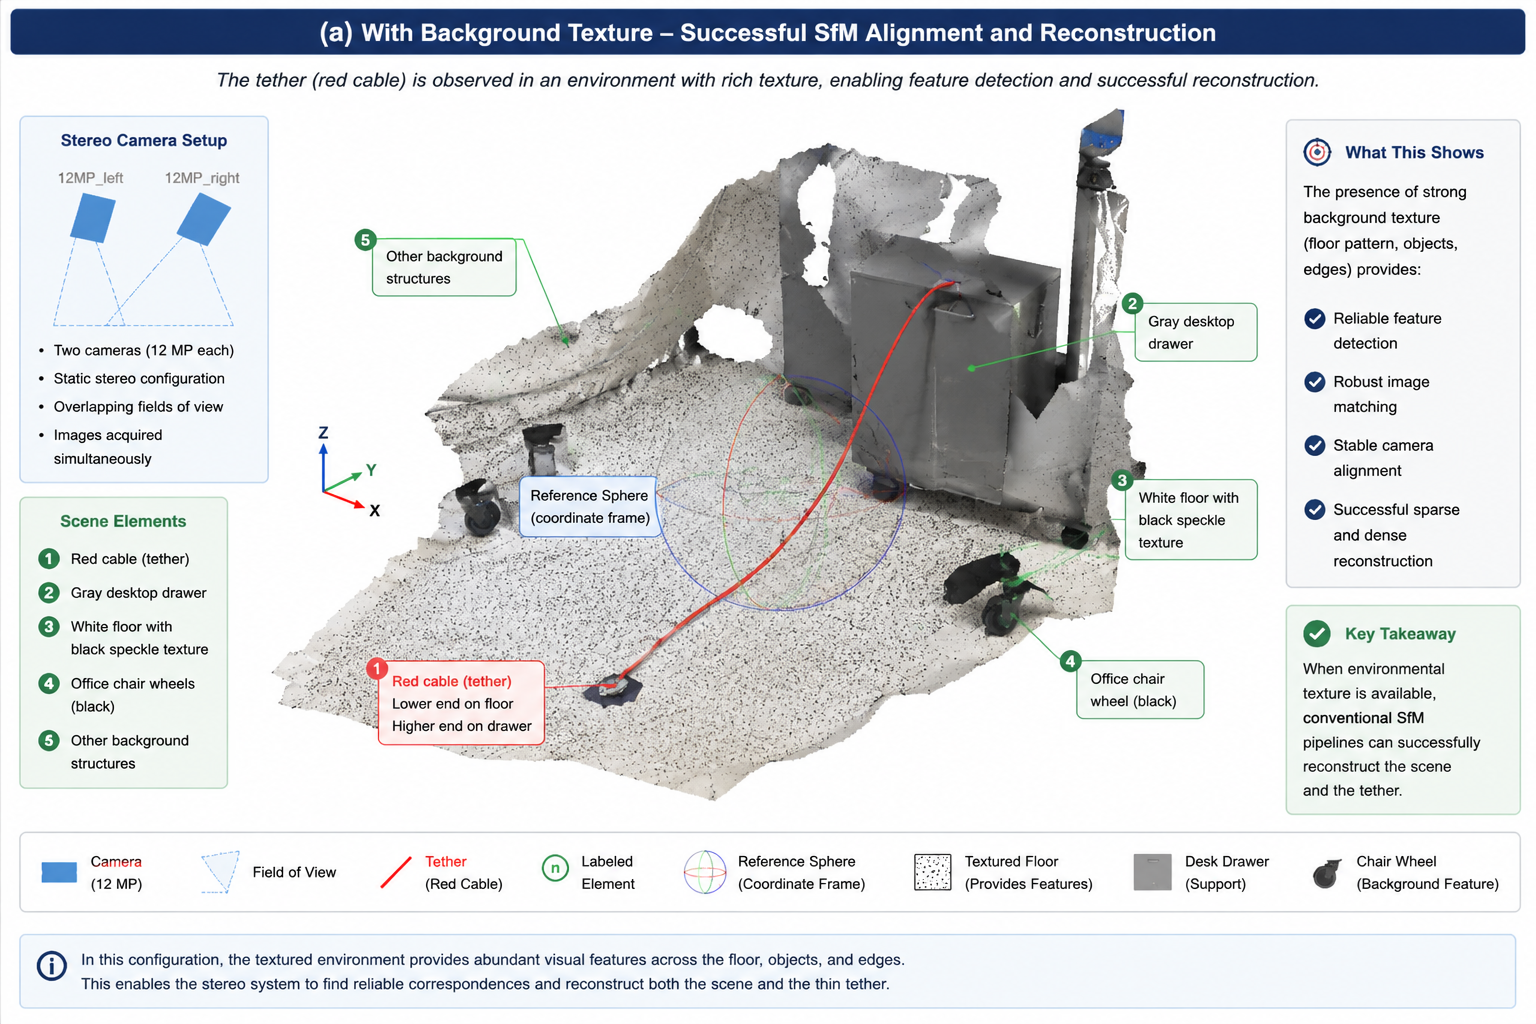
\includegraphics[width=\textwidth]{Images/Figure 6.3.png}
    \caption[Structure-from-Motion reconstruction supported by environmental texture features.]{Structure-from-Motion reconstruction supported by environmental texture features.}
    \label{fig:figure6.3}
\end{figure}

To evaluate the intrinsic reconstructability of the tether, a second experiment was performed in which the background was intentionally removed through image segmentation prior to processing. The resulting stereo pair retained only the isolated tether masks, eliminating the influence of environmental texture and ensuring that the reconstruction process relied exclusively on the visual information contained within the tether itself.
\\\\
The outcome of this experiment is shown in Figure \ref{fig:figure6.4}. Despite the successful isolation of the tether, the SfM pipeline failed to generate a valid reconstruction and returned a "Zero Resolution" error. No reliable camera alignment, sparse point cloud, or three-dimensional model could be obtained. This failure occurred even though the background had already been removed, eliminating the possibility that environmental structures or disparity artifacts could influence the reconstruction process.

\begin{figure}[!ht]
    \centering
    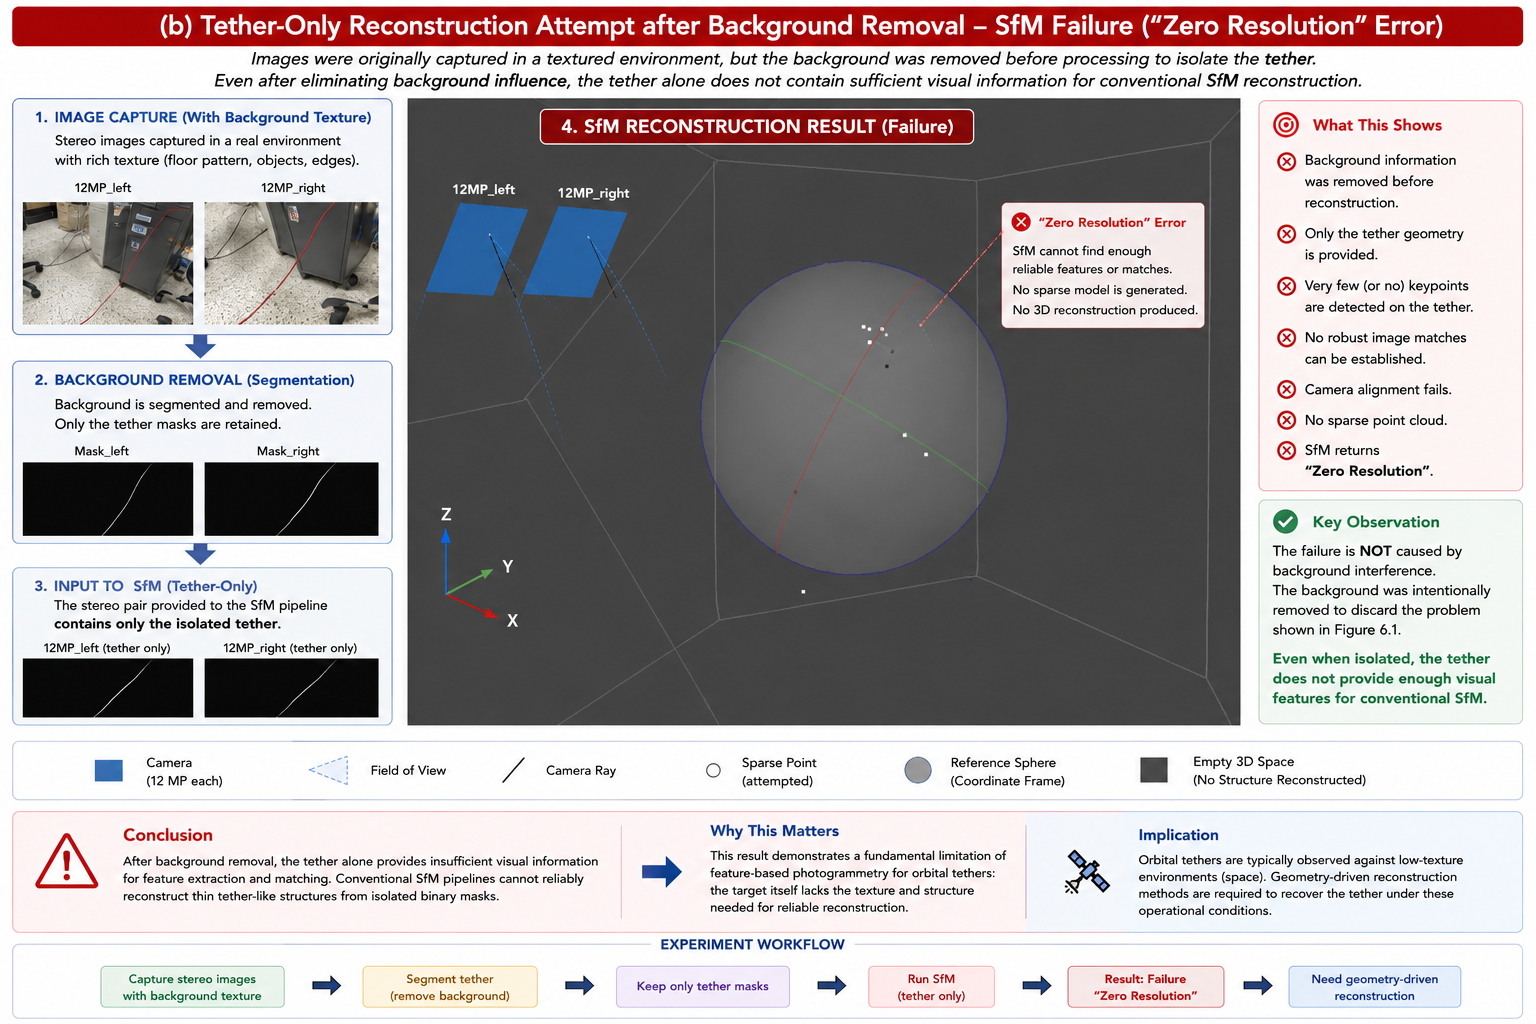
\includegraphics[width=\textwidth]{Images/Figure 6.4.png}
    \caption[Tether-only reconstruction attempt resulting in a ``Zero resolution'' failure.]{Tether-only reconstruction attempt resulting in a ``Zero resolution'' failure.}
    \label{fig:figure6.4}
\end{figure}

The results demonstrate that the primary limitation is not background interference but insufficient visual information within the tether itself. As a thin, elongated structure occupying only a small number of pixels in each image, the tether provides very few distinctive keypoints for conventional feature-extraction and matching algorithms. Consequently, the correspondence stage becomes underconstrained, preventing robust image alignment and subsequent three-dimensional reconstruction.
\\\\
The comparison between Figures \ref{fig:figure6.3} and \ref{fig:figure6.4} provides direct experimental evidence of a fundamental limitation of conventional feature-based photogrammetry. While SfM can successfully reconstruct scenes with abundant environmental texture, it cannot reliably reconstruct an isolated tether even after perfect segmentation. Therefore, the reconstruction challenge is not merely a segmentation problem but a structural limitation of feature-based approaches when applied to thin, low-texture objects.
\\\\
These observations directly motivate the geometry-driven reconstruction methodology introduced in Chapter \ref{chap:theoretical-optical-analyses}. Rather than relying on sparse image features, the proposed approach exploits radiometric localization, centerline estimation, geometric continuity constraints, and stereo correspondence strategies specifically designed for thin tether-like structures operating under low-texture orbital observation conditions.

\subsection{Implications for orbital tether observation}
The results presented in Sections \ref{sub:volumetric-object-reconstruction} and \ref{sub:tether-reconstruction-failure}  reveal two complementary limitations of conventional photogrammetric reconstruction when applied to orbital tether observation.
\\\\
The dense stereo reconstruction experiment demonstrated that disparity-based methods remain highly sensitive to the absence of environmental texture. Although portions of the target geometry could be recovered, substantial phantom structures and false correspondences were generated throughout regions that physically correspond to empty space. The resulting reconstructions required extensive manual filtering and could not be considered operationally autonomous.
\\\\
The Structure-from-Motion evaluation exposed an even more fundamental limitation. In the case of the tether proxy, the reconstruction process failed because the target itself did not provide sufficient visual features to support reliable feature extraction and image matching. As environmental texture was progressively removed, the reconstruction quality degraded until complete failure occurred.
\\\\
These observations are consistent with the optical analysis presented in Chapter \ref{chap:theoretical-optical-analyses}. Under orbital observation conditions, tether visibility is governed not only by geometric sampling but also by radiometric contrast, directional illumination, and sub-pixel detectability effects. Consequently, the tether cannot be treated as a conventional textured object suitable for feature-based photogrammetry across a significant portion of the operational range.
\\\\
The experimental evidence therefore motivates the transition toward the geometry-driven reconstruction methodology introduced in Chapter \ref{chap:experimental-processing-approaches}. Rather than relying on sparse image features, the proposed approach exploits radiometric signatures, geometric continuity, centerline estimation, and stereo correspondence constraints specifically adapted to thin tether-like structures. This strategy directly addresses the limitations observed in conventional photogrammetric reconstruction and provides the foundation for the results presented in the following sections.

\section{Geometry-driven reconstruction results}

The geometry-driven reconstruction methodology introduced in Chapter \ref{chap:experimental-processing-approaches} was evaluated using the tether datasets described in Section \ref{sec:validation-objectives-experimental-datasets}, after establishing the limitations of conventional photogrammetric methods in Section \ref{sec:evaluation-conventional-photogrammetry}. The objective was to determine whether geometric and radiometric constraints could provide reliable tether reconstruction under low-texture conditions where conventional feature-based approaches failed.
\\\\
Two representative tether configurations were analyzed, as shown in Figures \ref{fig:figureplanar} and \ref{fig:figure3d}. Scenario A corresponds to a predominantly planar configuration, in which the tether is arranged approximately parallel to the image plane and exhibits limited depth variation. Scenario B introduces stronger out-of-plane deformation, looped geometry, and depth variation, thereby representing a more demanding reconstruction case.

\begin{figure}[!ht]
    \centering
    \begin{subfigure}{0.48\textwidth}
        \centering
        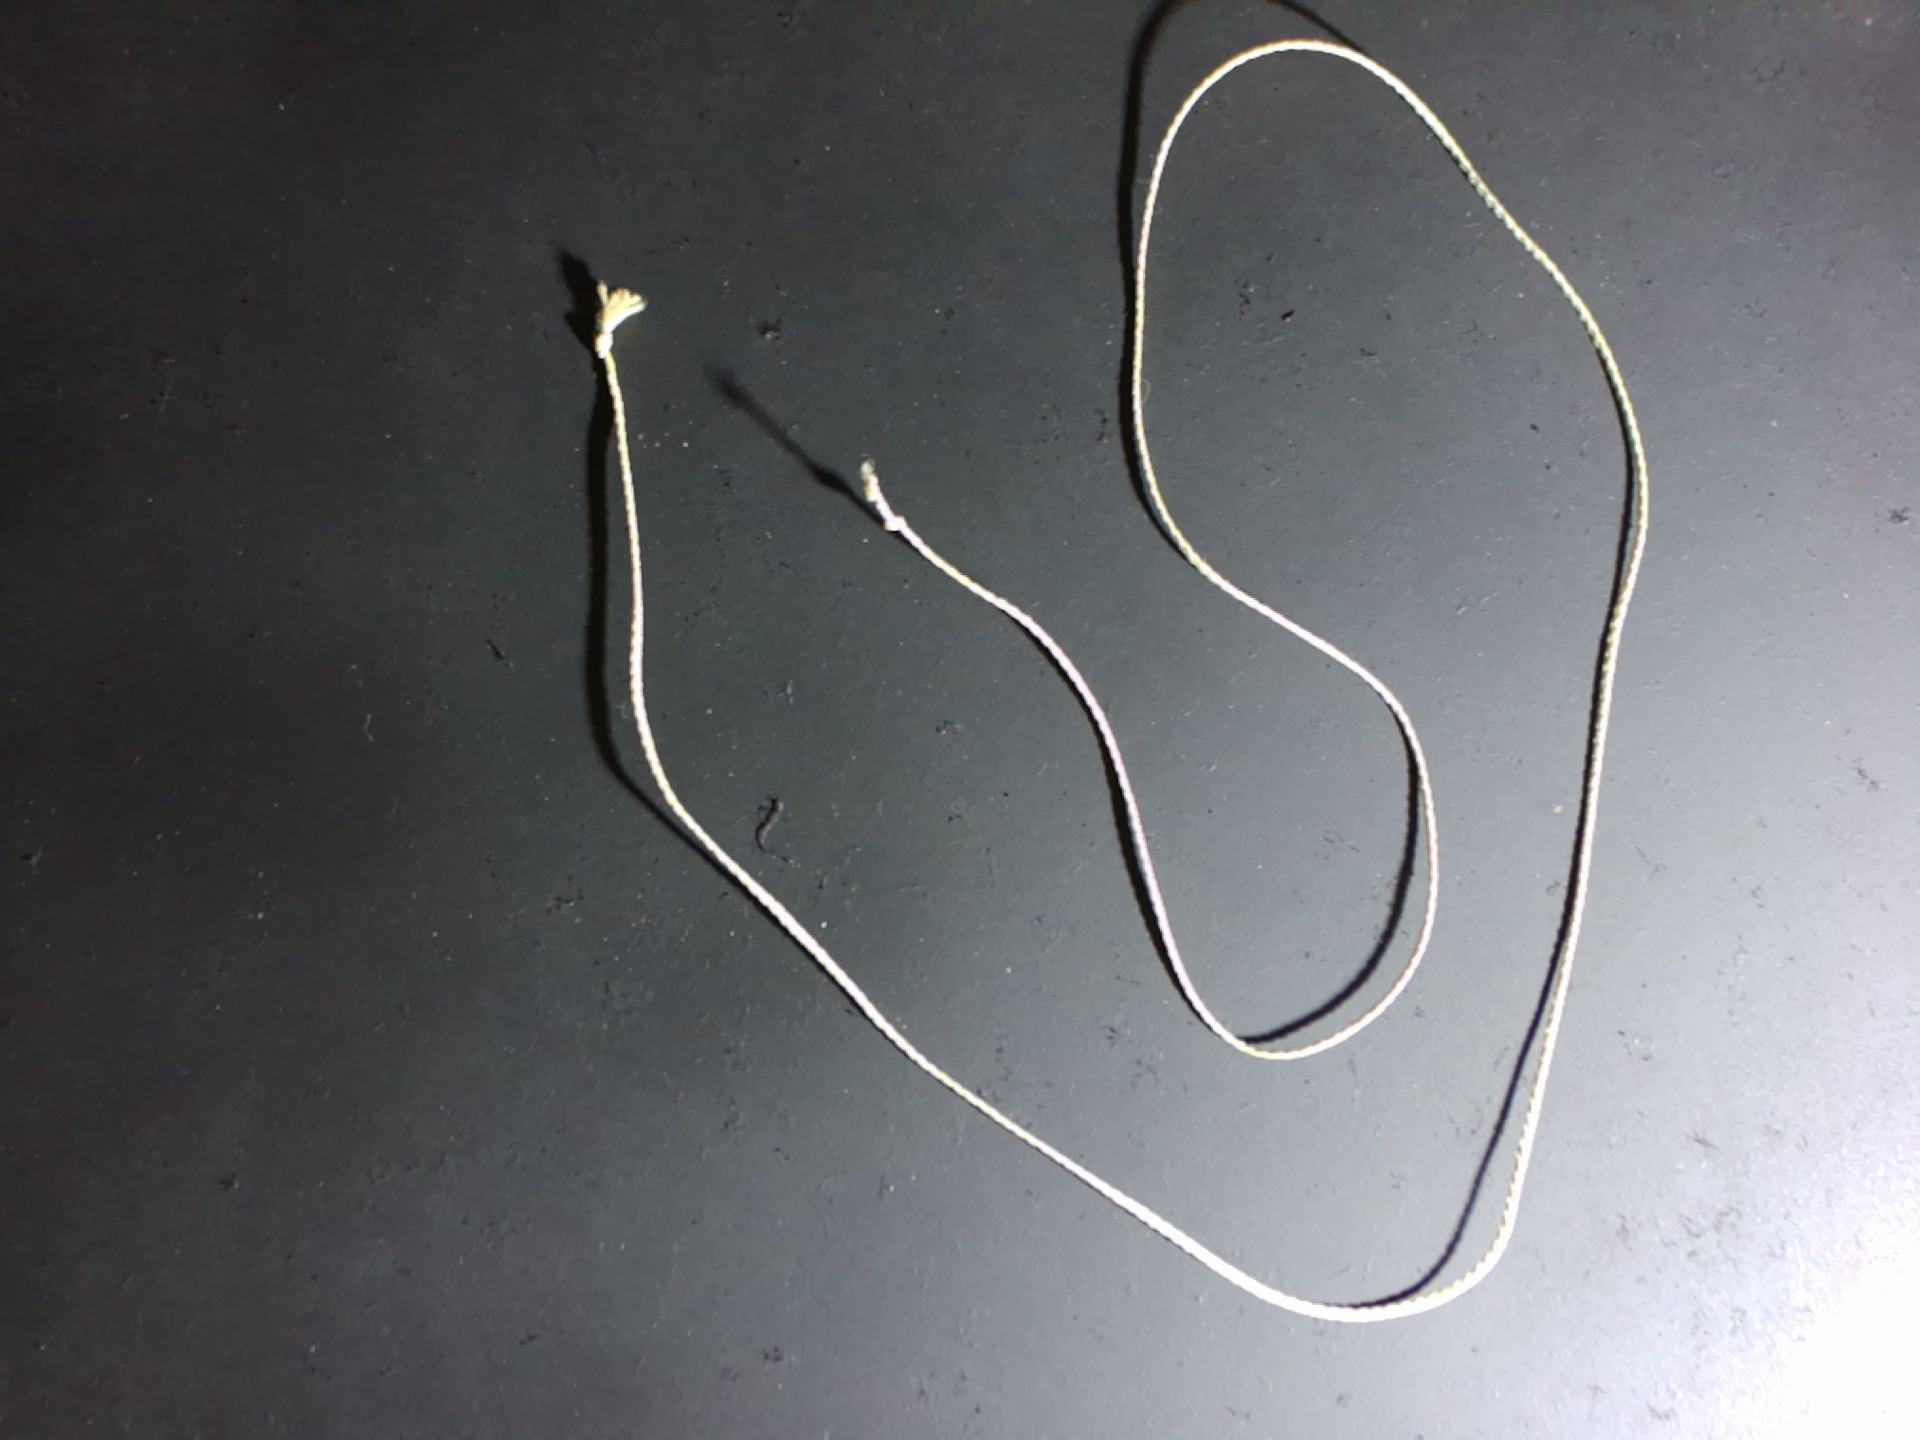
\includegraphics[height=5cm]{Images/Figureplanar.jpg}
        \caption{Scenario A - Tether proxy positioned on the XY plane inside the dark enclosure.}
        \label{fig:figureplanar}
    \end{subfigure}
    \hfill
    \begin{subfigure}{0.48\textwidth}
        \centering
        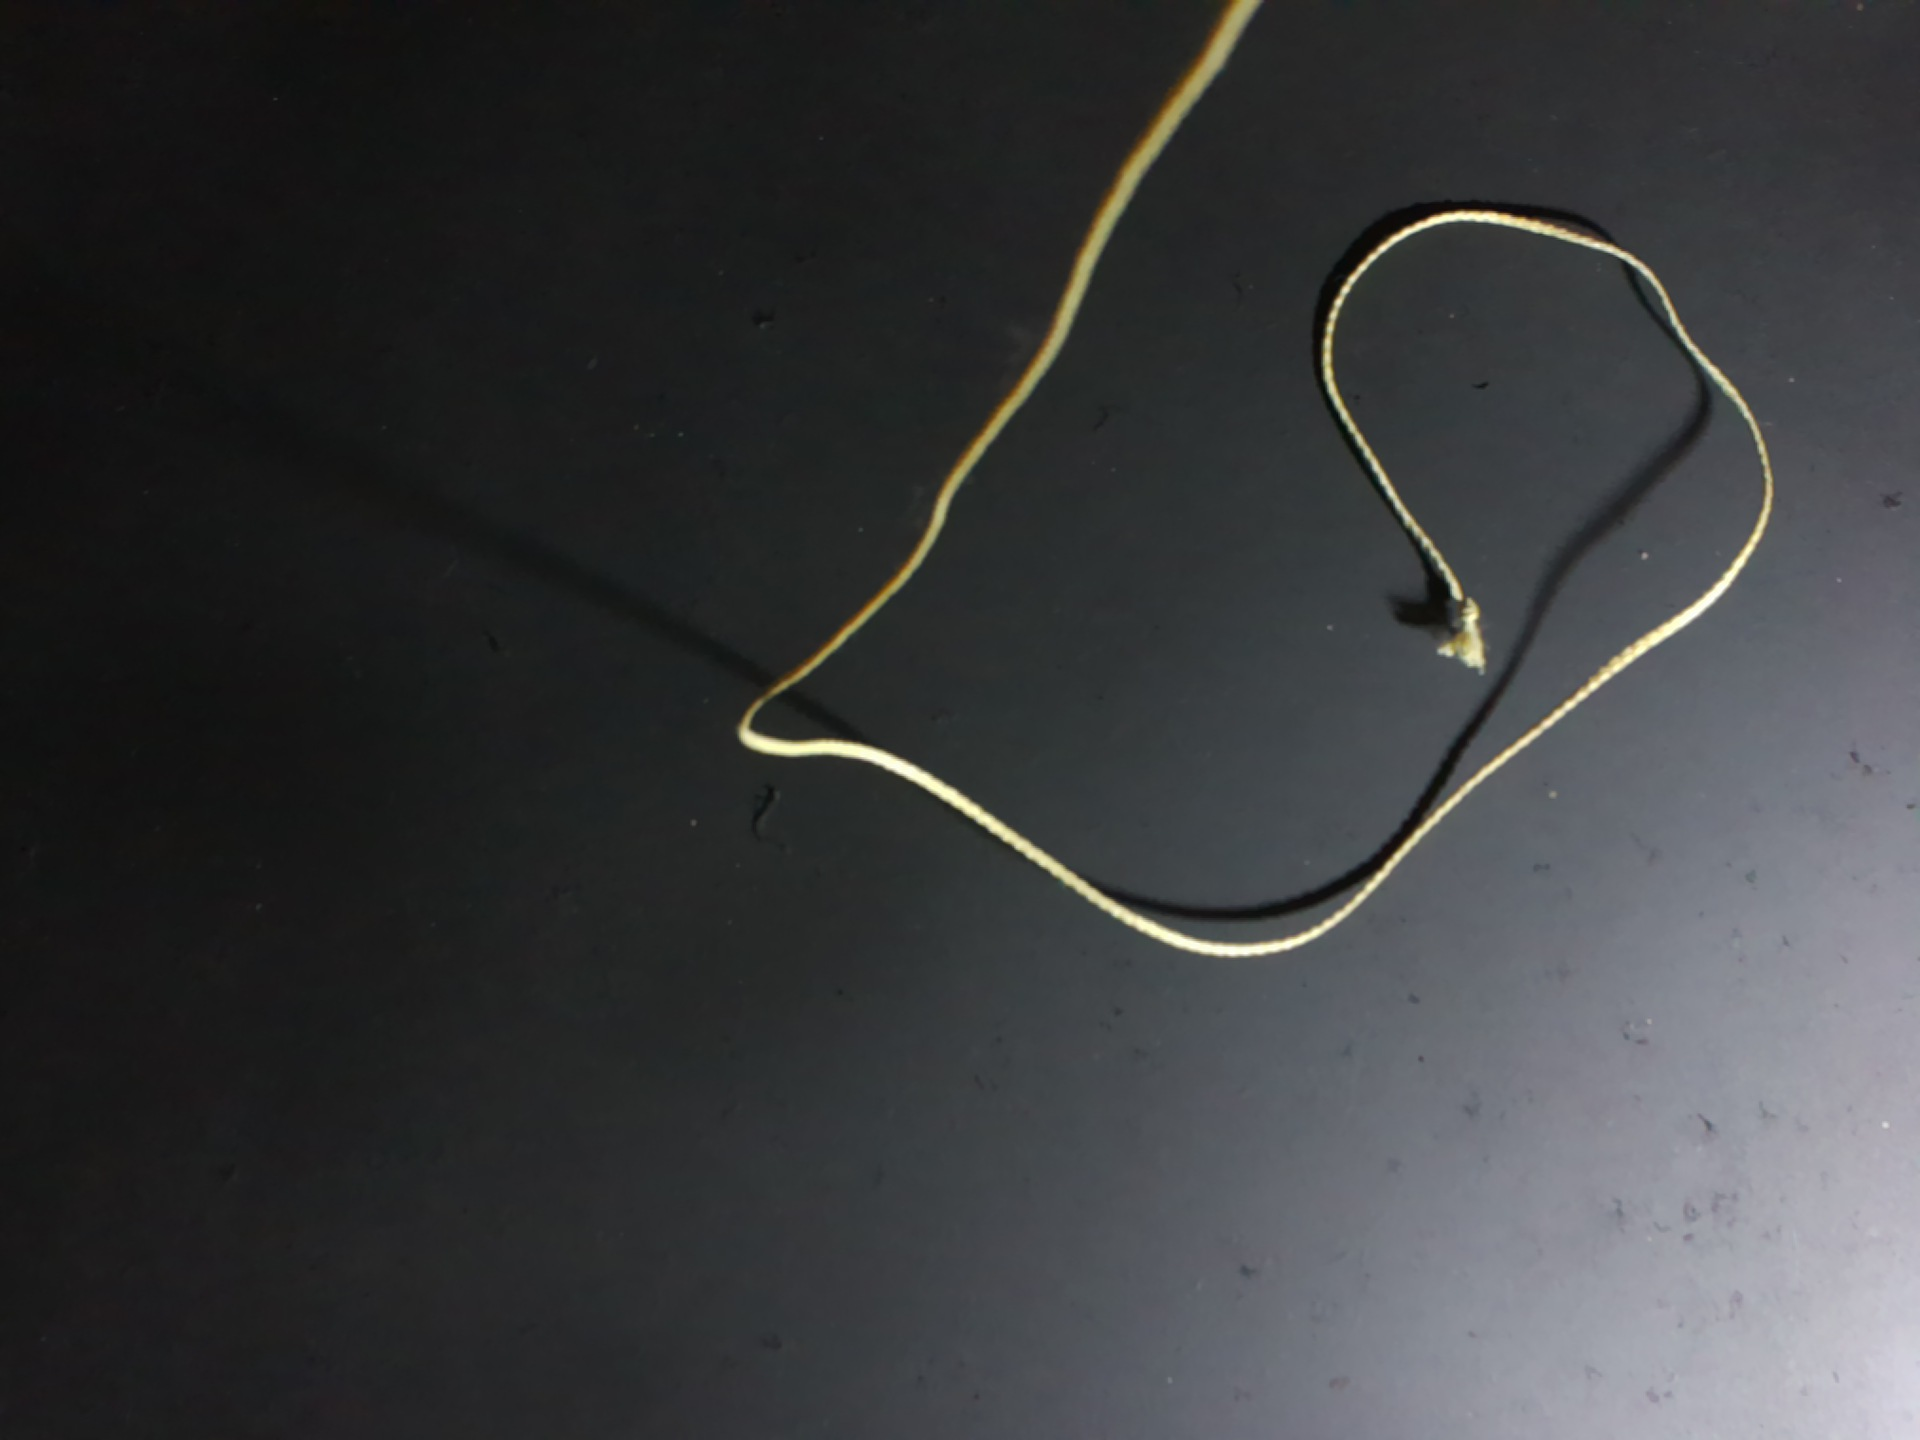
\includegraphics[height=5cm]{Images/Figure3d.jpg}
        \caption{Scenario B - Tether proxy with one end elevated relative to the XY plane inside the dark enclosure.}
        \label{fig:figure3d}
    \end{subfigure}
    \caption{Experimental Scenarios A and B for validating the geometry-driven tether reconstruction process.}
    \label{fig:scenarios}
\end{figure}

For clarity, the results are presented by experimental scenario. Each scenario is analyzed through the same reconstruction sequence: tether extraction, stereo correspondence establishment, and three-dimensional reconstruction. This organization allows the complete reconstruction process to be evaluated first for the simpler planar case and then for the more complex volumetric case.

\subsection{Reconstruction Workflow for Scenario A}

Scenario A was used to evaluate the performance of the geometry-driven reconstruction framework under a predominantly planar tether configuration. In this case, the expected depth variation is limited, and the stereo displacement between corresponding tether points should remain relatively uniform.
\\\\
The first processing stage consisted of extracting the tether from the stereo image pair. As shown in Figure \ref{fig:figure6.5}, the tether was successfully isolated as a continuous binary trace in both the left and right images. The extracted curves preserve the principal topology of the tether and provide a clean geometric representation for subsequent correspondence analysis.

\begin{figure}[!ht]
    \centering
    \begin{minipage}{0.48\textwidth}
        \centering
        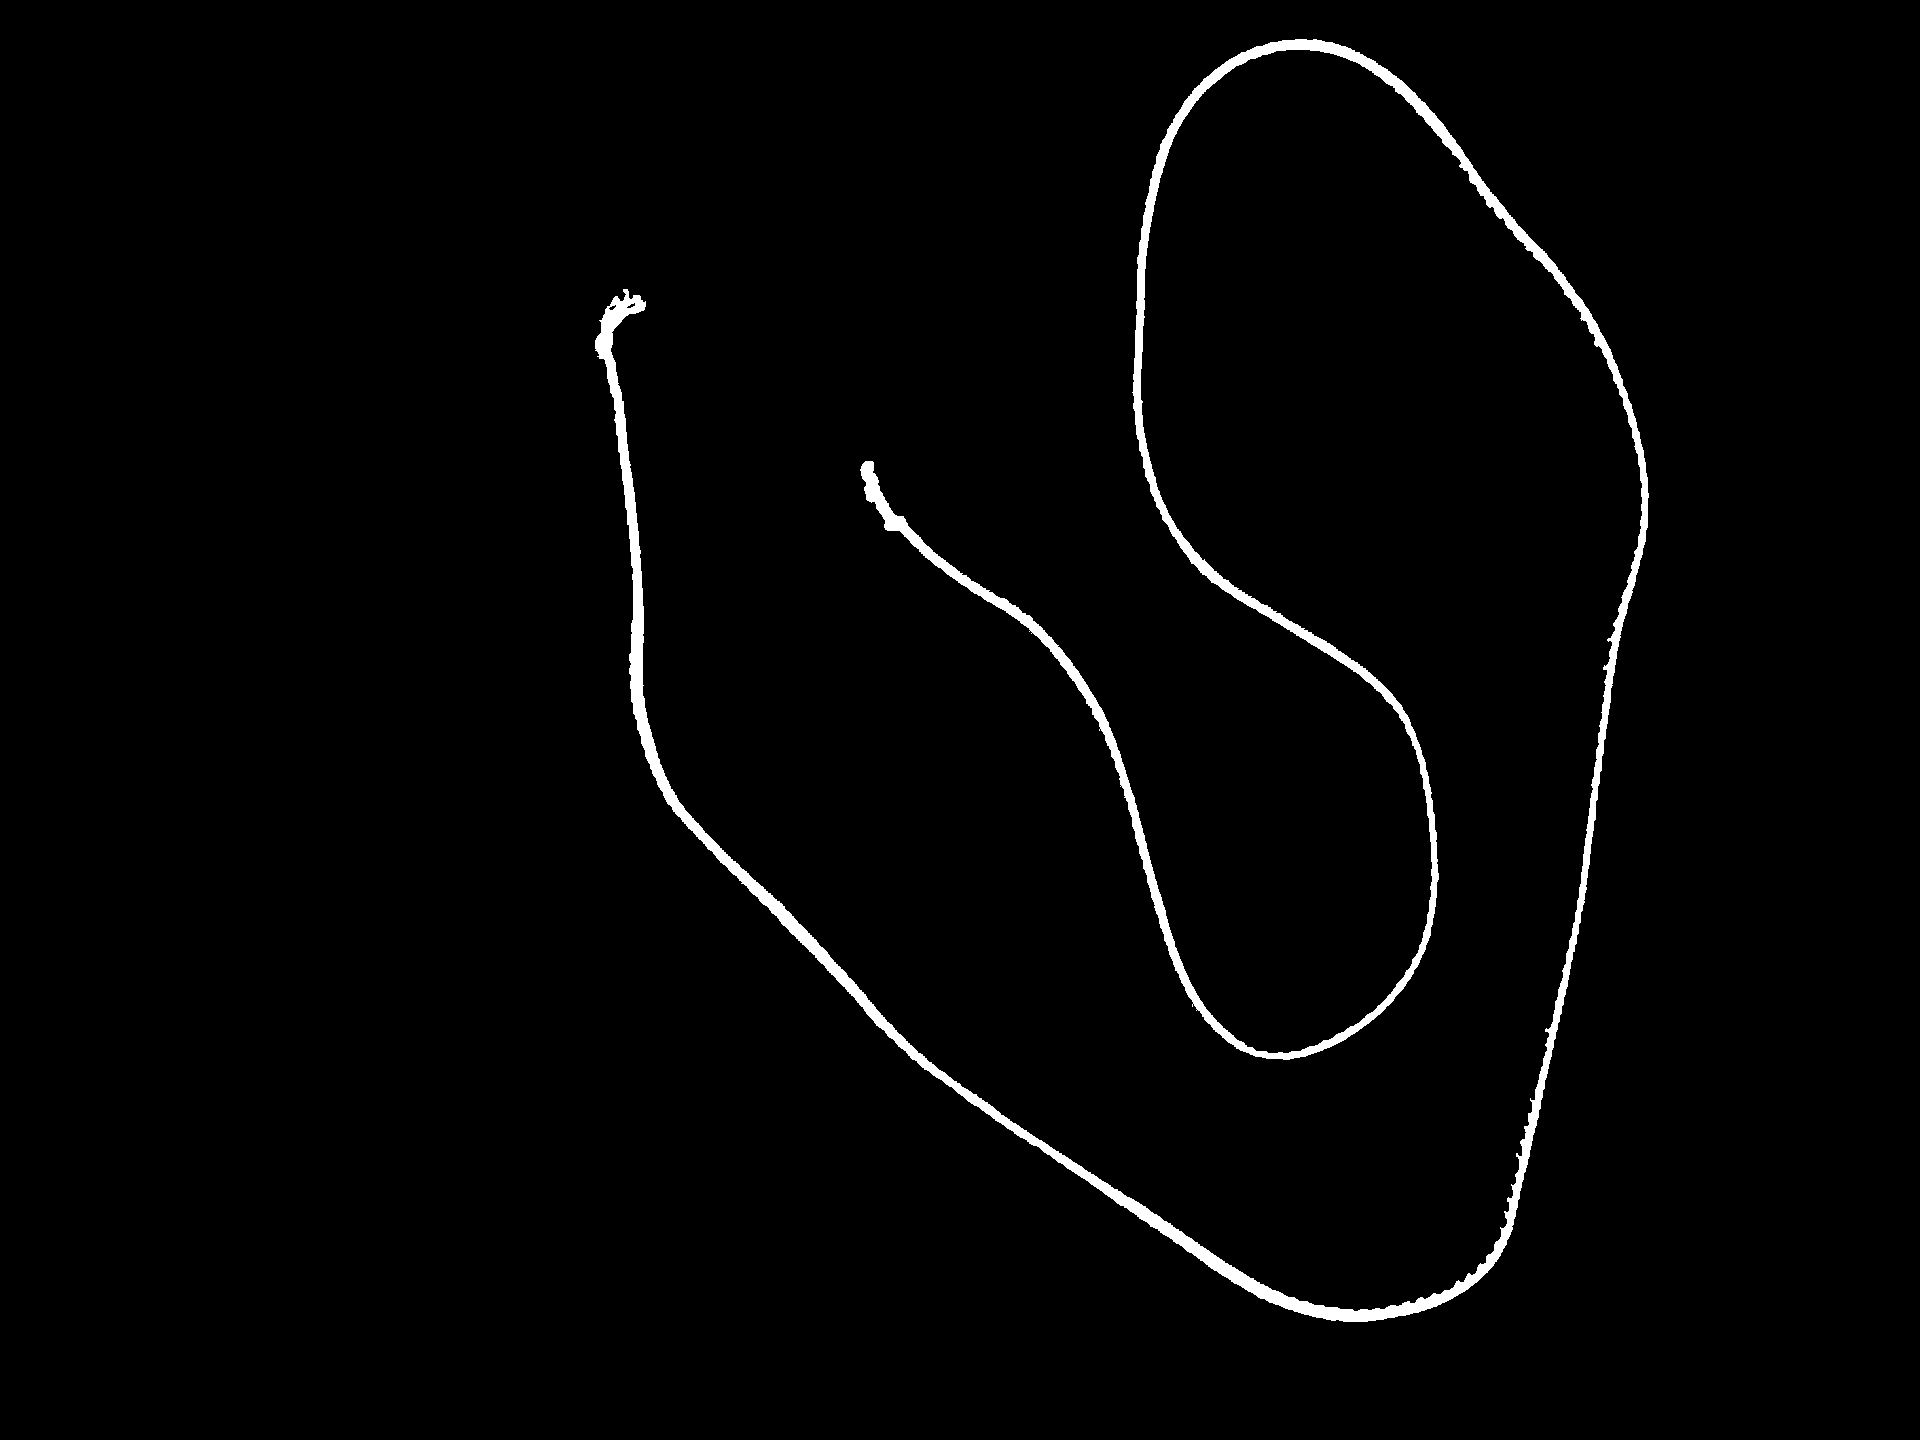
\includegraphics[width=\textwidth]{Images/Figure 6.5a.png}
    \end{minipage}
    \hfill
    \begin{minipage}{0.48\textwidth}
        \centering
        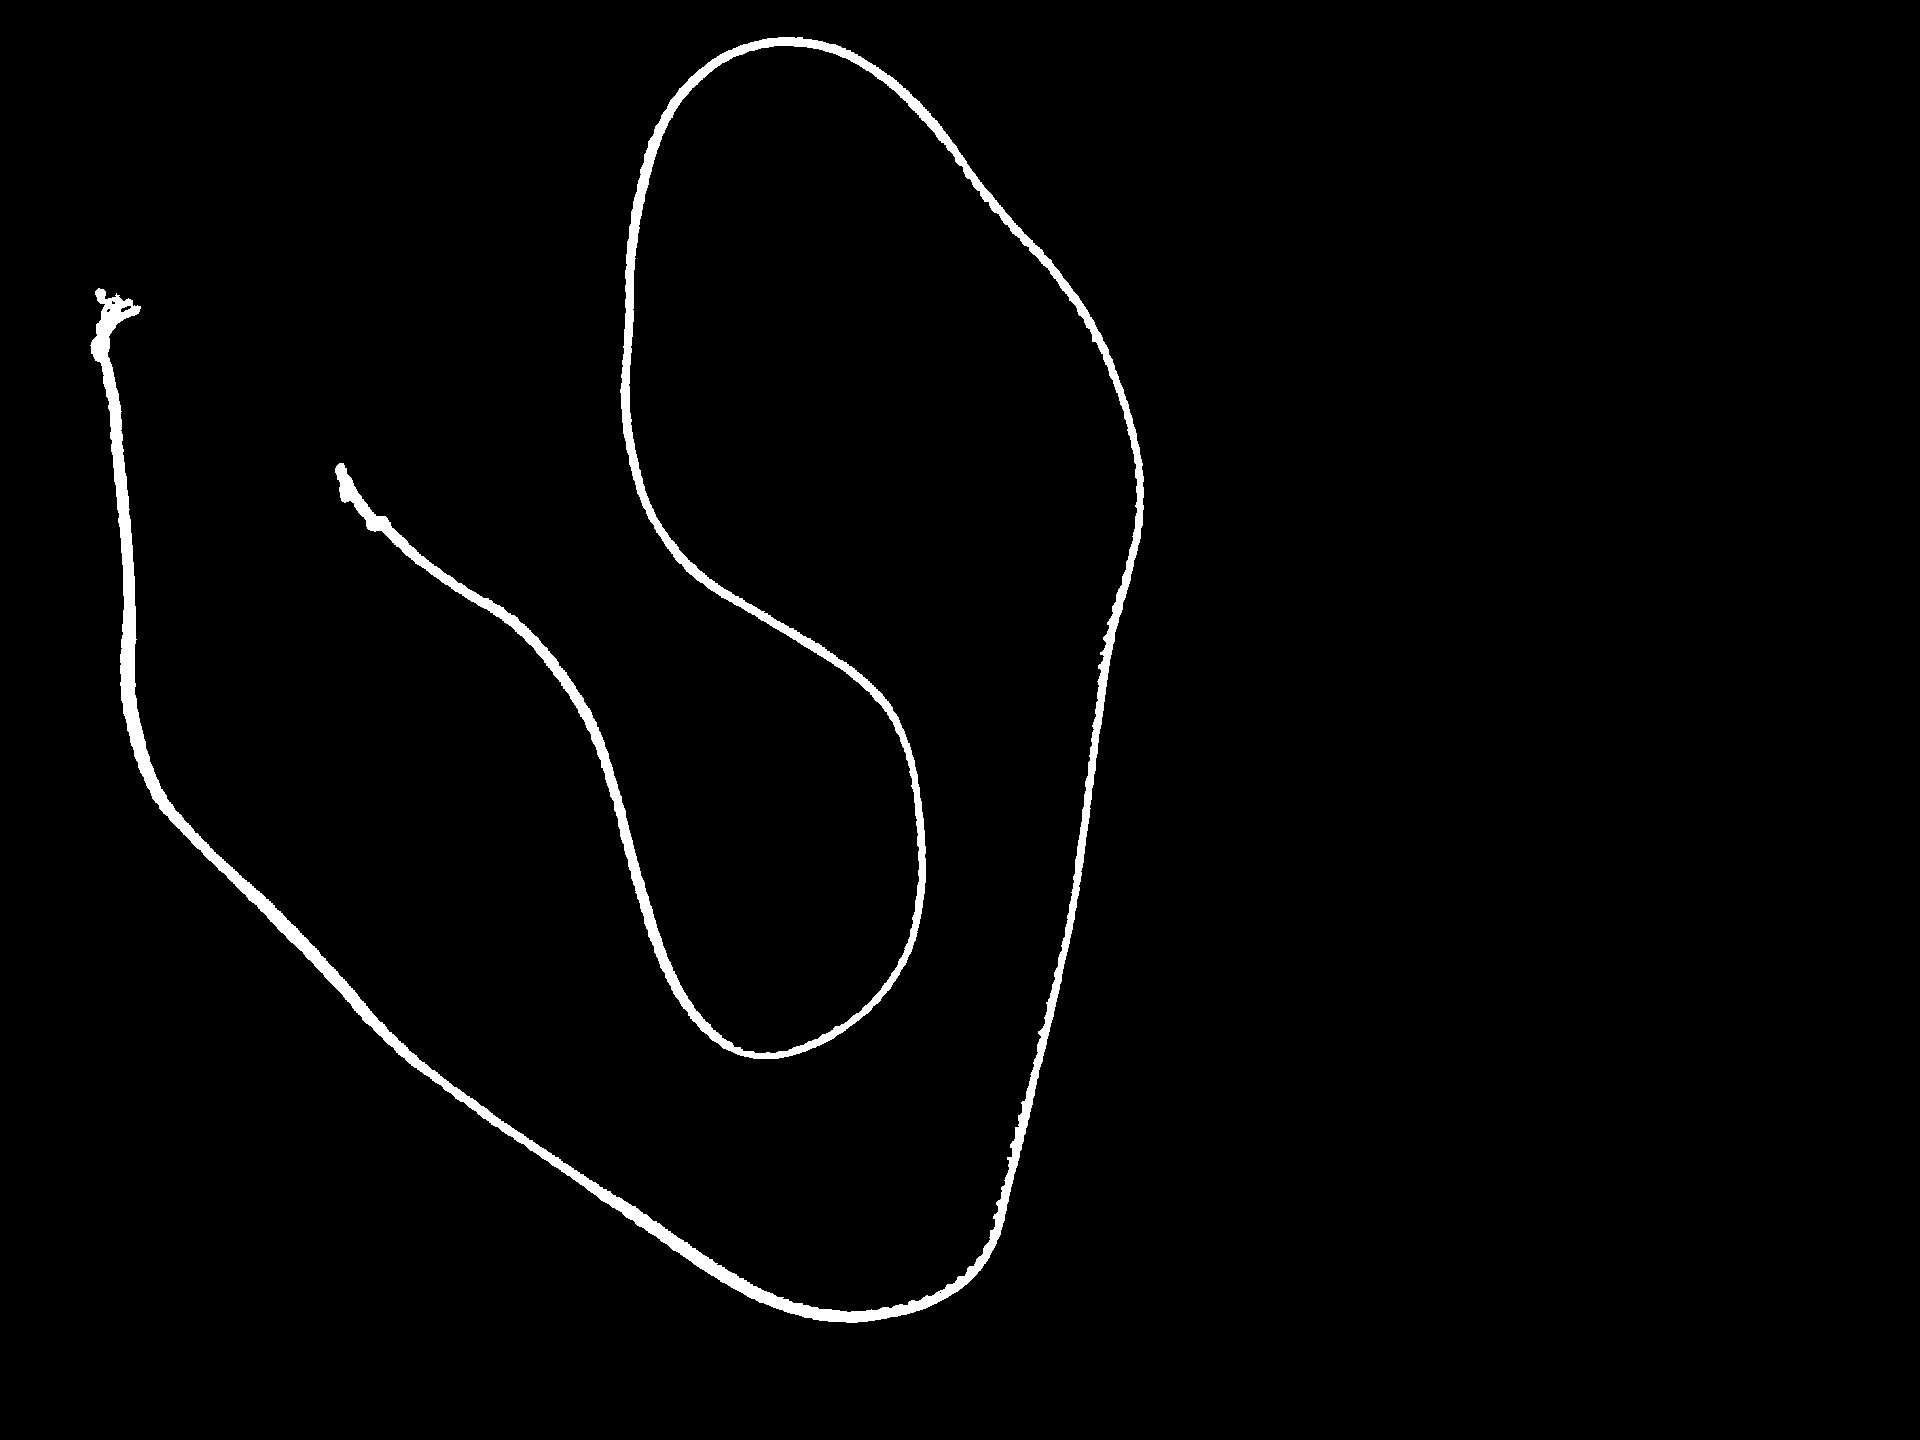
\includegraphics[width=\textwidth]{Images/Figure 6.5b.png}
    \end{minipage}
    \caption[Extraction results obtained for Scenario A]{(Left) left camera image, (Right) right camera image. Tether extraction results for Scenario A (planar geometry). The binary traces successfully isolate the thin structure against the black background with a relatively uniform horizontal shift.}
    \label{fig:figure6.5}
\end{figure}

After extraction, stereo correspondence was established between the left and right tether traces. Figure \ref{fig:figure6.7} shows that the matching lines are approximately parallel and relatively uniform, which is consistent with the limited depth variation of the planar configuration.

\begin{figure}[!ht]
    \centering
    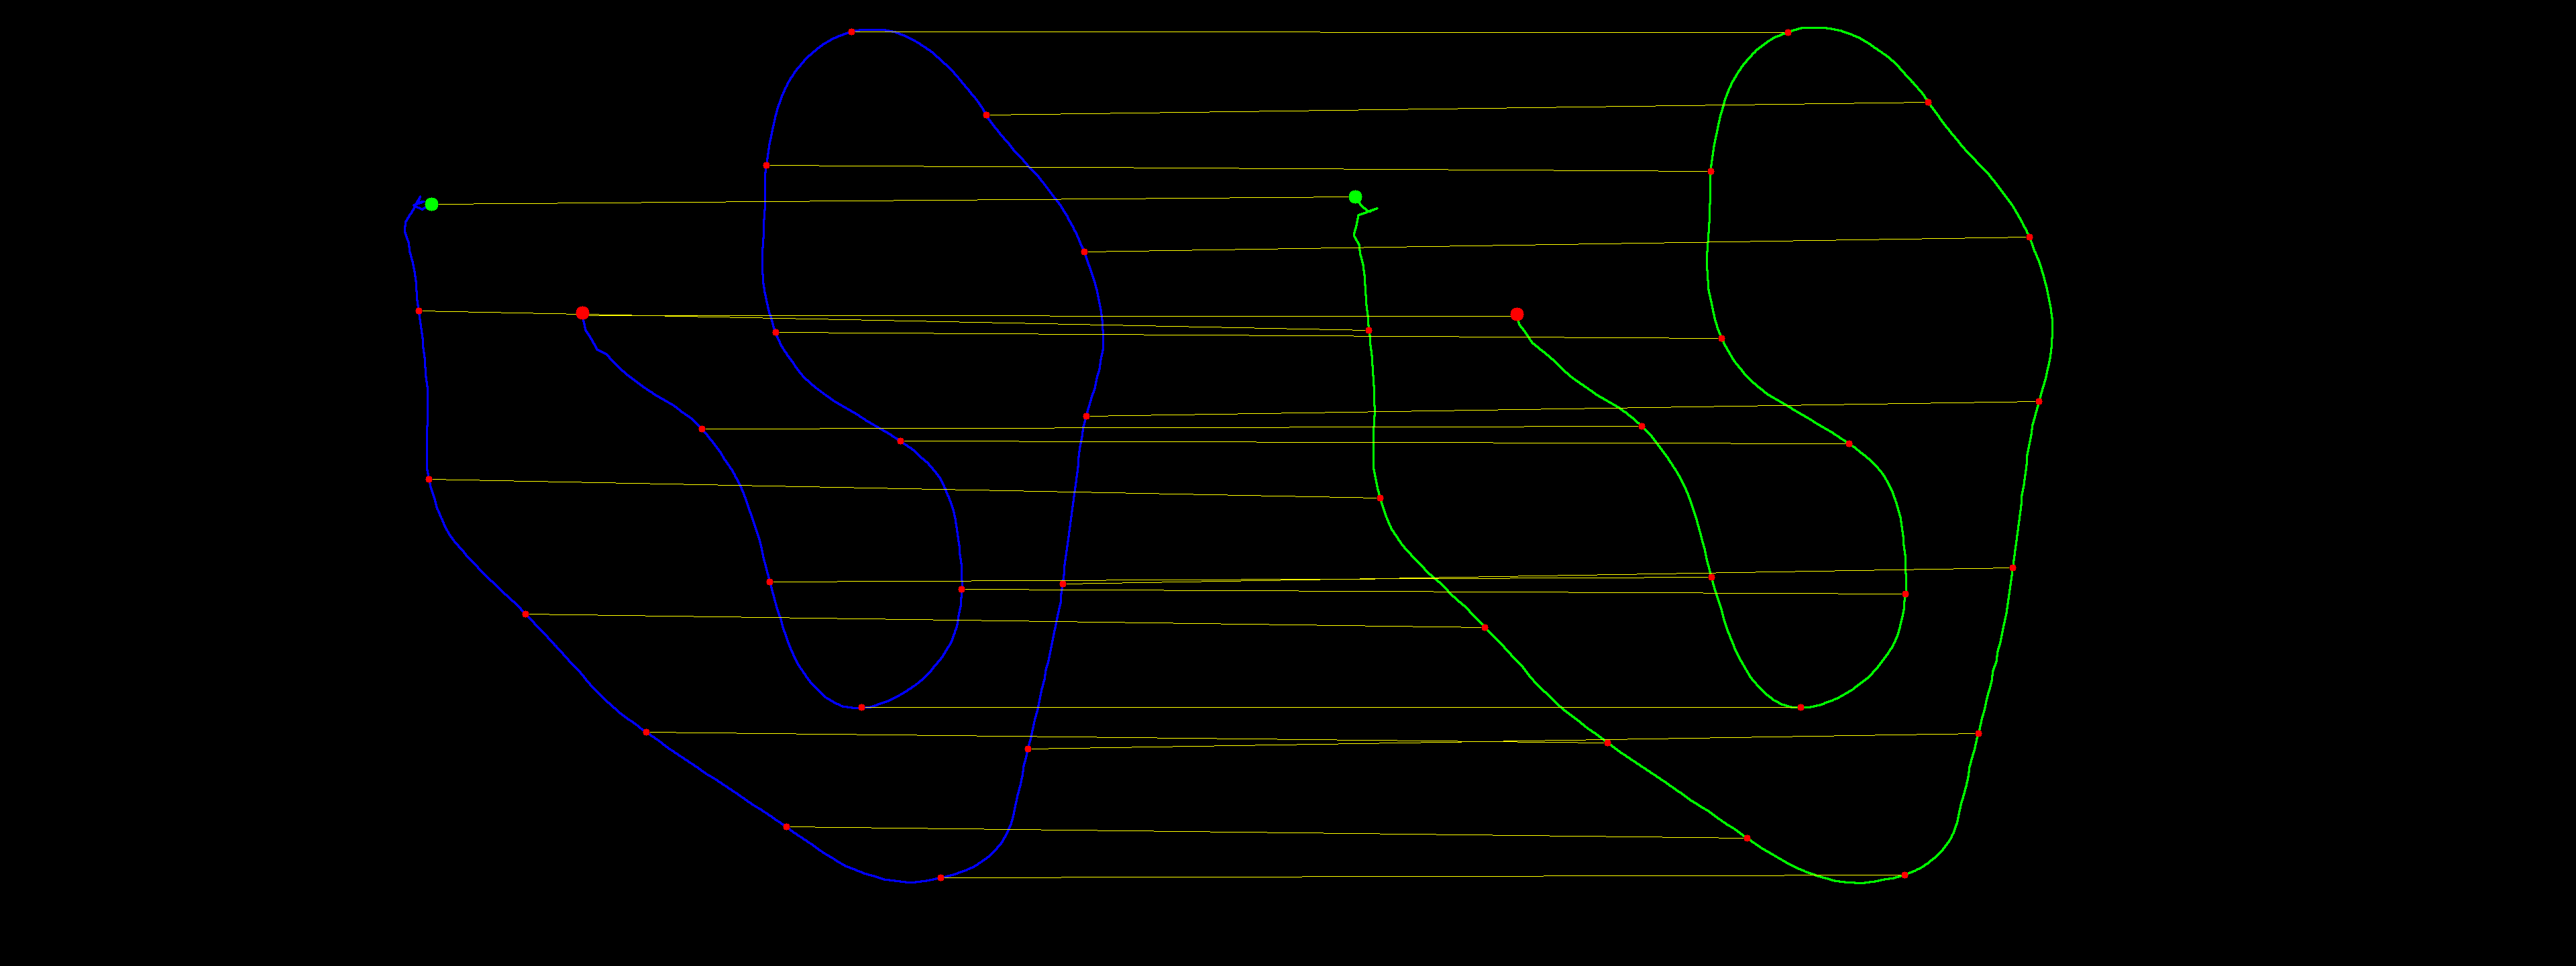
\includegraphics[width=\textwidth]{Images/Figure 6.7.png}
    \caption[Stereo correspondence results for Scenario A.]{Stereo correspondence results for Scenario A. The parallel and uniform matching lines indicate consistent depth across the planar geometry.}
    \label{fig:figure6.7}
\end{figure}

The matched tether points were then triangulated to recover the three-dimensional tether trajectory. Figure \ref{fig:figure6.9} presents the final 3D reconstruction obtained for Scenario A. The reconstructed geometry preserves the overall shape of the tether and confirms that the proposed method can recover spatially coherent tether trajectories without relying on environmental texture or conventional feature matching.

\begin{figure}[!ht]
    \centering
    \begin{minipage}{0.48\textwidth}
        \centering
        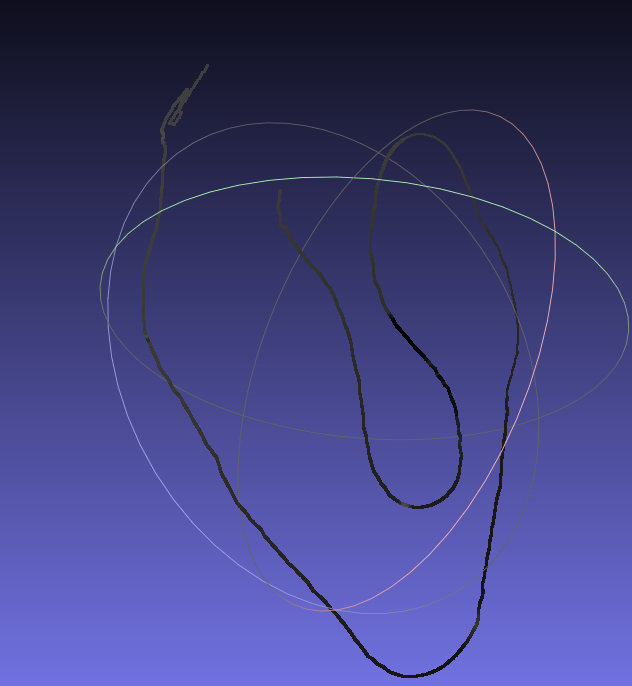
\includegraphics[height=7cm]{Images/Figure 6.9a.png}
    \end{minipage}
    \hfill
    \begin{minipage}{0.48\textwidth}
        \centering
        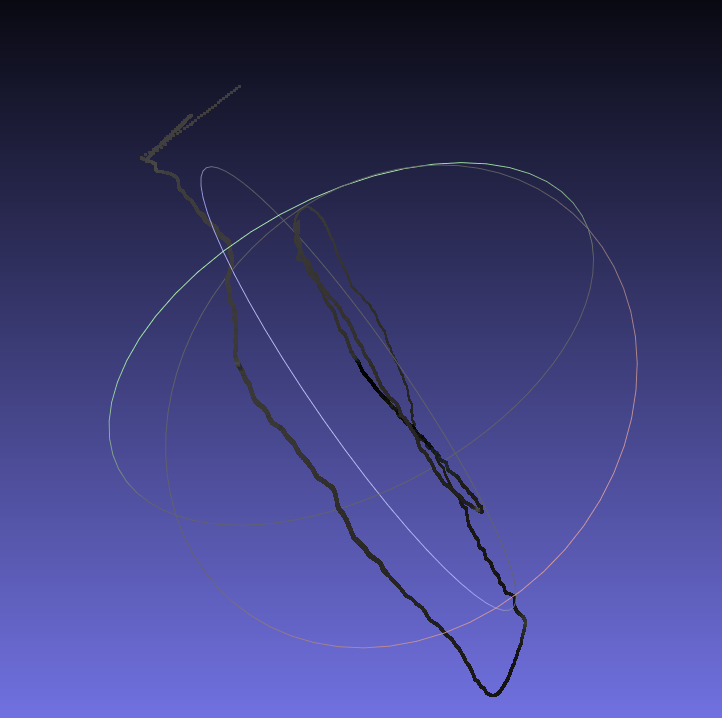
\includegraphics[height=7cm]{Images/Figure 6.9b.png}
    \end{minipage}
    \caption[Final three-dimensional tether reconstruction for Scenario A.]{Final three-dimensional tether reconstruction for Scenario A. The spatial coherence confirms successful triangulation of a relatively flat geometry.}
    \label{fig:figure6.9}
\end{figure}

The complete reconstruction sequence for Scenario A is summarized in Figure \ref{fig:figure6.11}, which integrates the stereo image pair, extracted traces, correspondence results, and final 3D representation.

\begin{figure}[!ht]
    \centering
    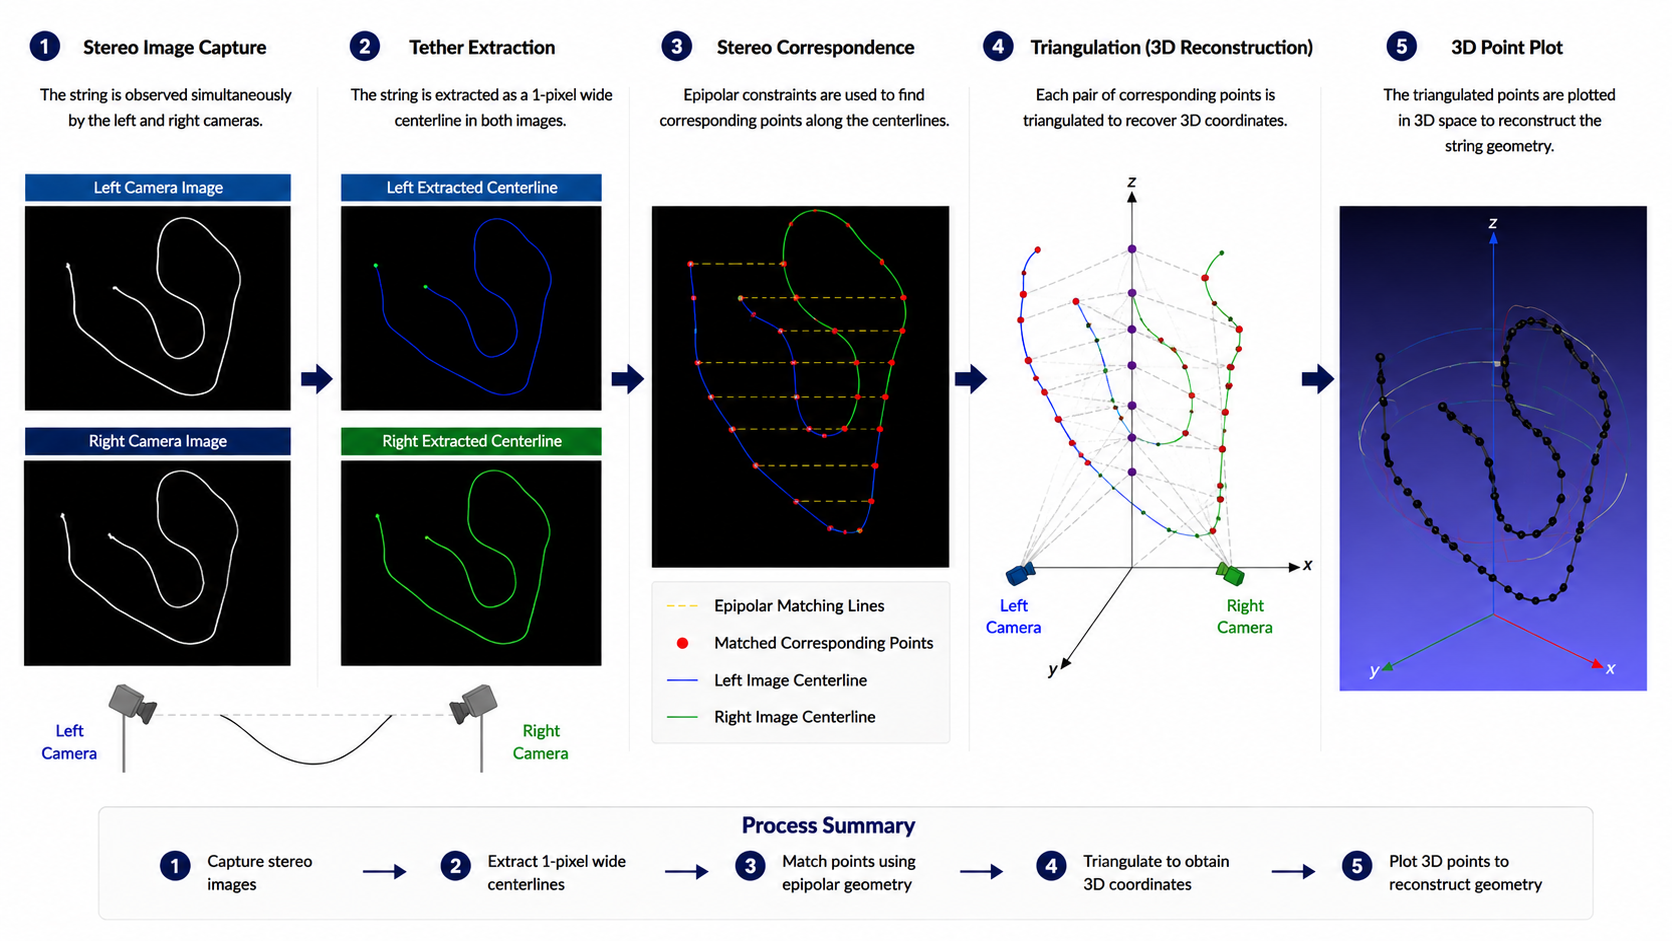
\includegraphics[width=\textwidth]{Images/Figure 6.11.png}
    \caption[Geometry-driven stereo reconstruction workflow from image capture to three-dimensional tether representation in scenario A.]{Geometry-driven Stereo reconstruction workflow from image capture to three-dimensional tether representation in scenario A.}
    \label{fig:figure6.11}
\end{figure}

\subsection{Reconstruction Workflow for Scenario B}

Scenario B was used to evaluate the robustness of the geometry-driven reconstruction framework under a more complex tether configuration. Unlike Scenario A, this case includes out-of-plane deformation, perspective foreshortening, and stronger depth variation along the tether.
\\\\
The first processing stage again consisted of tether extraction from the stereo image pair. As shown in Figure \ref{fig:figure6.6}, the method was able to isolate continuous tether traces in both camera views despite the increased geometric complexity. The extracted curves preserve the main shape of the tether, including looped and deformed regions.

\begin{figure}[!ht]
    \centering
    \begin{minipage}{0.48\textwidth}
        \centering
        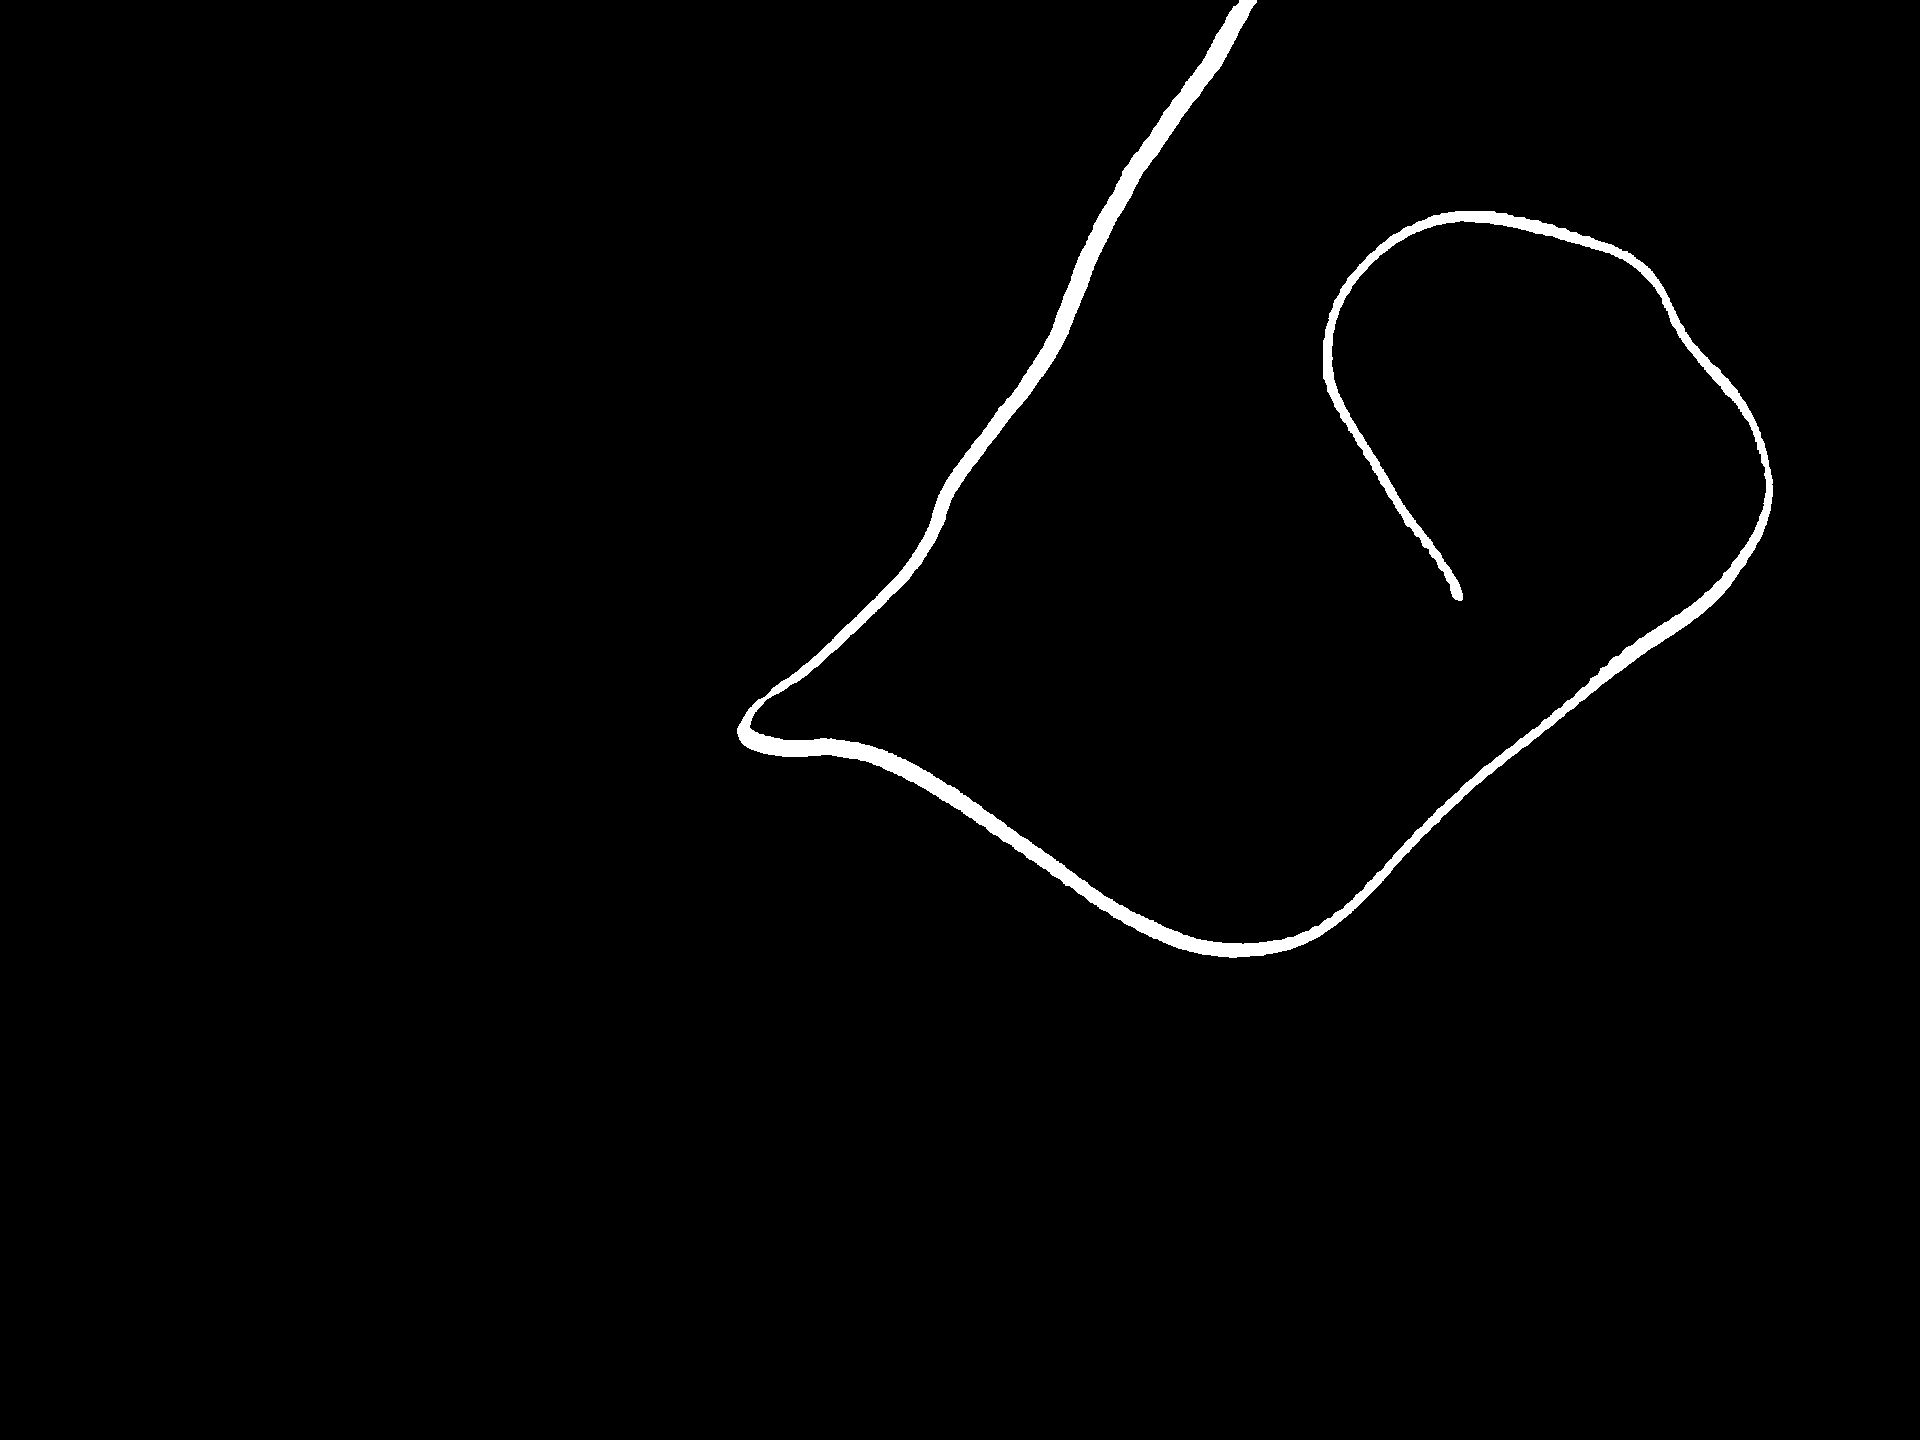
\includegraphics[width=\textwidth]{Images/Figure 6.6a.png}
    \end{minipage}
    \hfill
    \begin{minipage}{0.48\textwidth}
        \centering
        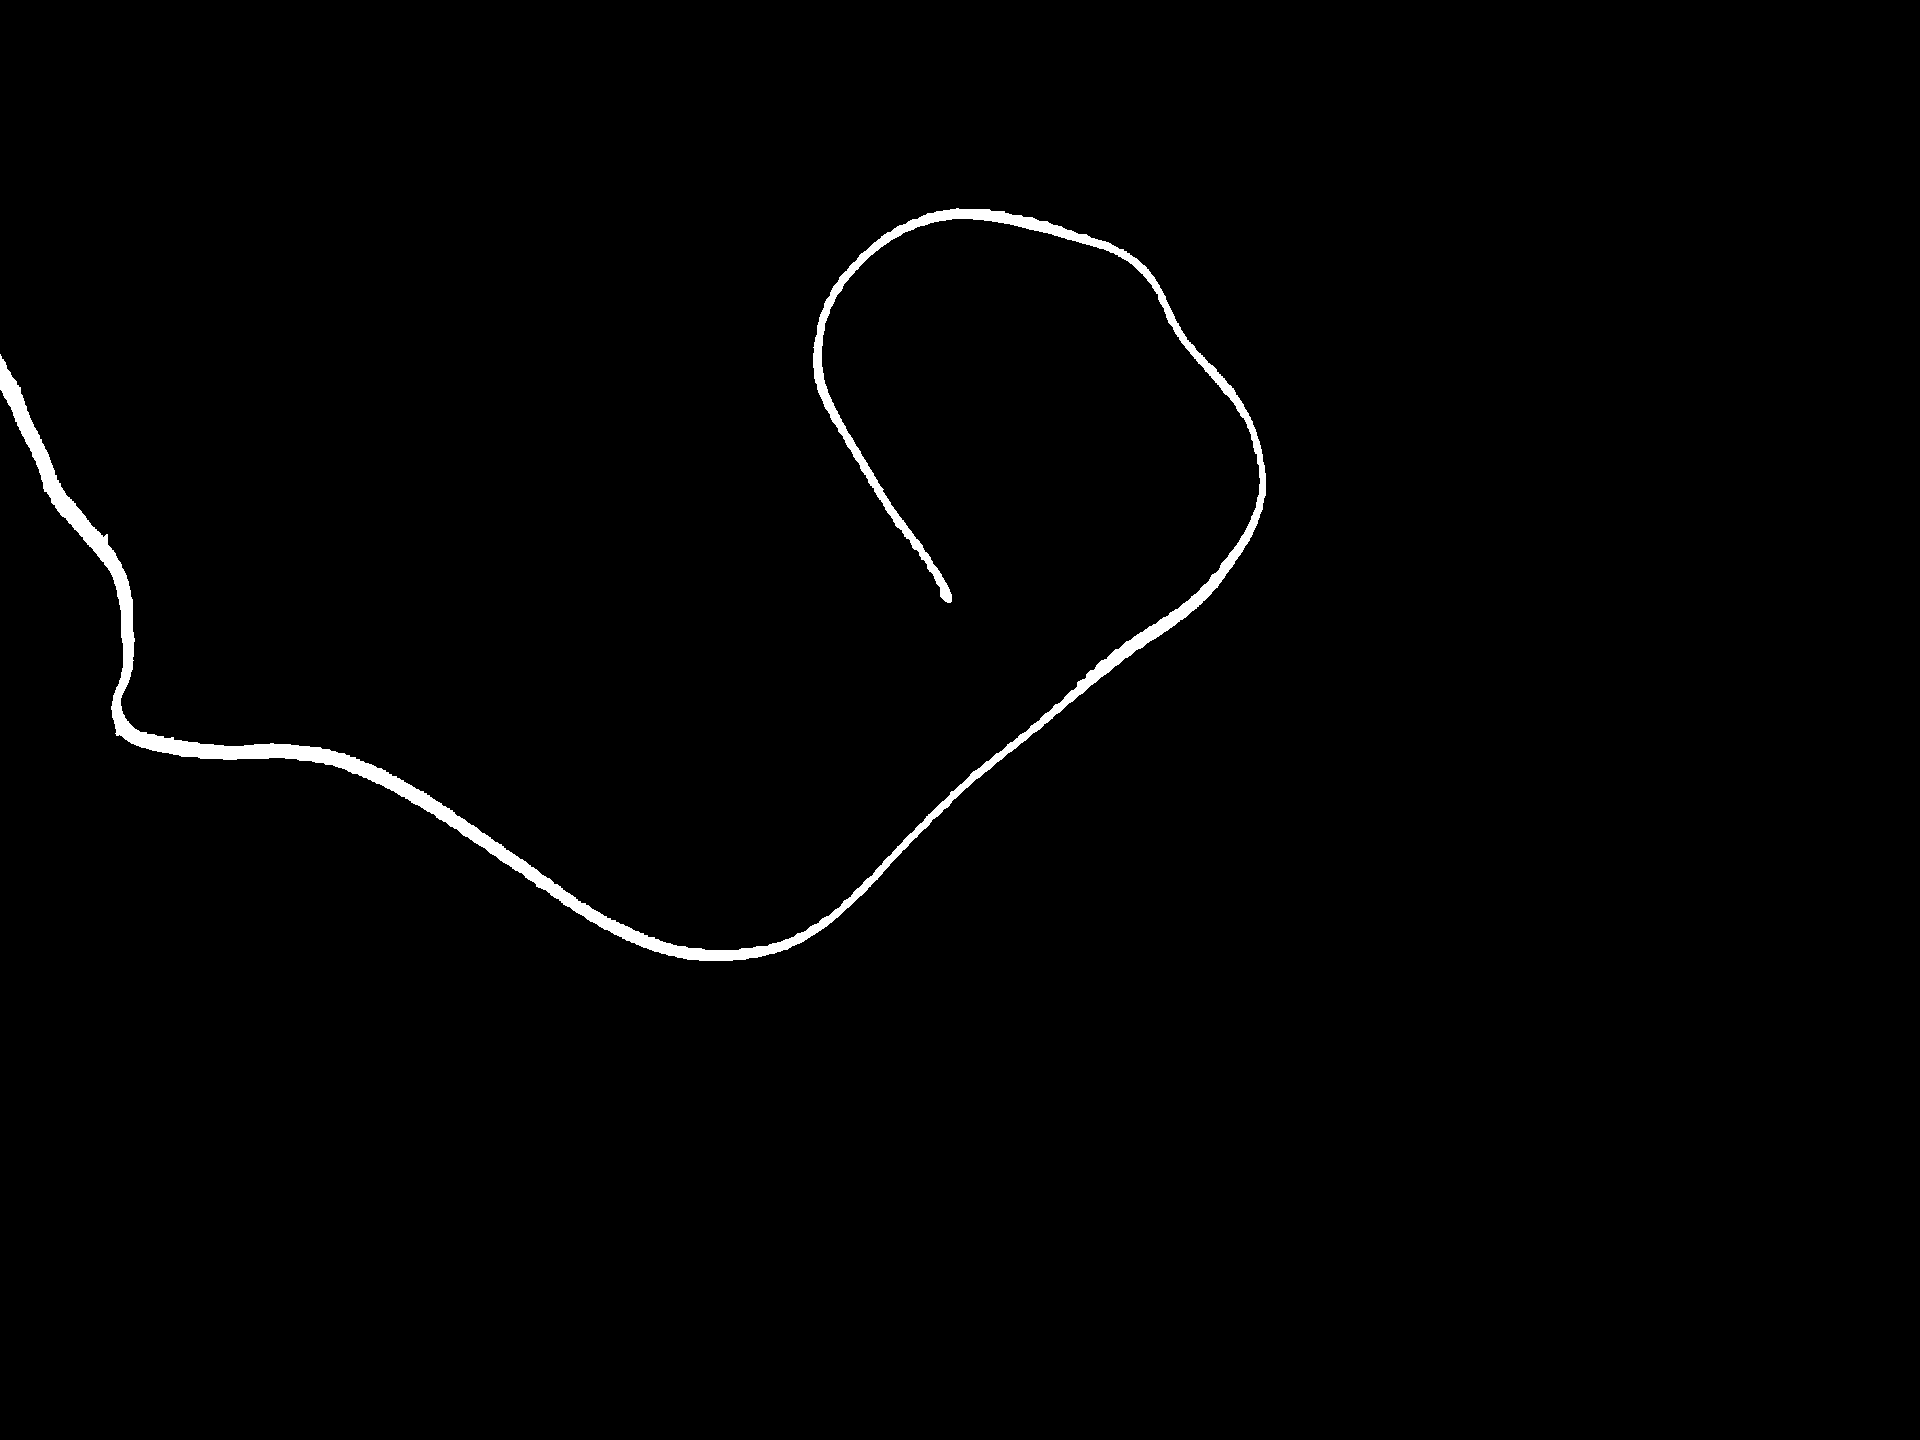
\includegraphics[width=\textwidth]{Images/Figure 6.6b.png}
    \end{minipage}
    \caption[Extraction results obtained for Scenario B]{(Left) left camera image, (Right) right camera image. Tether extraction results for Scenario B (volumetric geometry). The algorithm maintains continuous trace extraction despite the complex loops and perspective foreshortening caused by the tether extending toward the camera lenses.}
    \label{fig:figure6.6}
\end{figure}

Stereo correspondence was then established between the left and right extracted traces. Figure \ref{fig:figure6.8} shows that the matching lines exhibit more variable lengths than in Scenario A. This behavior is consistent with the stronger depth variation present in the volumetric configuration.

\begin{figure}[!ht]
    \centering
    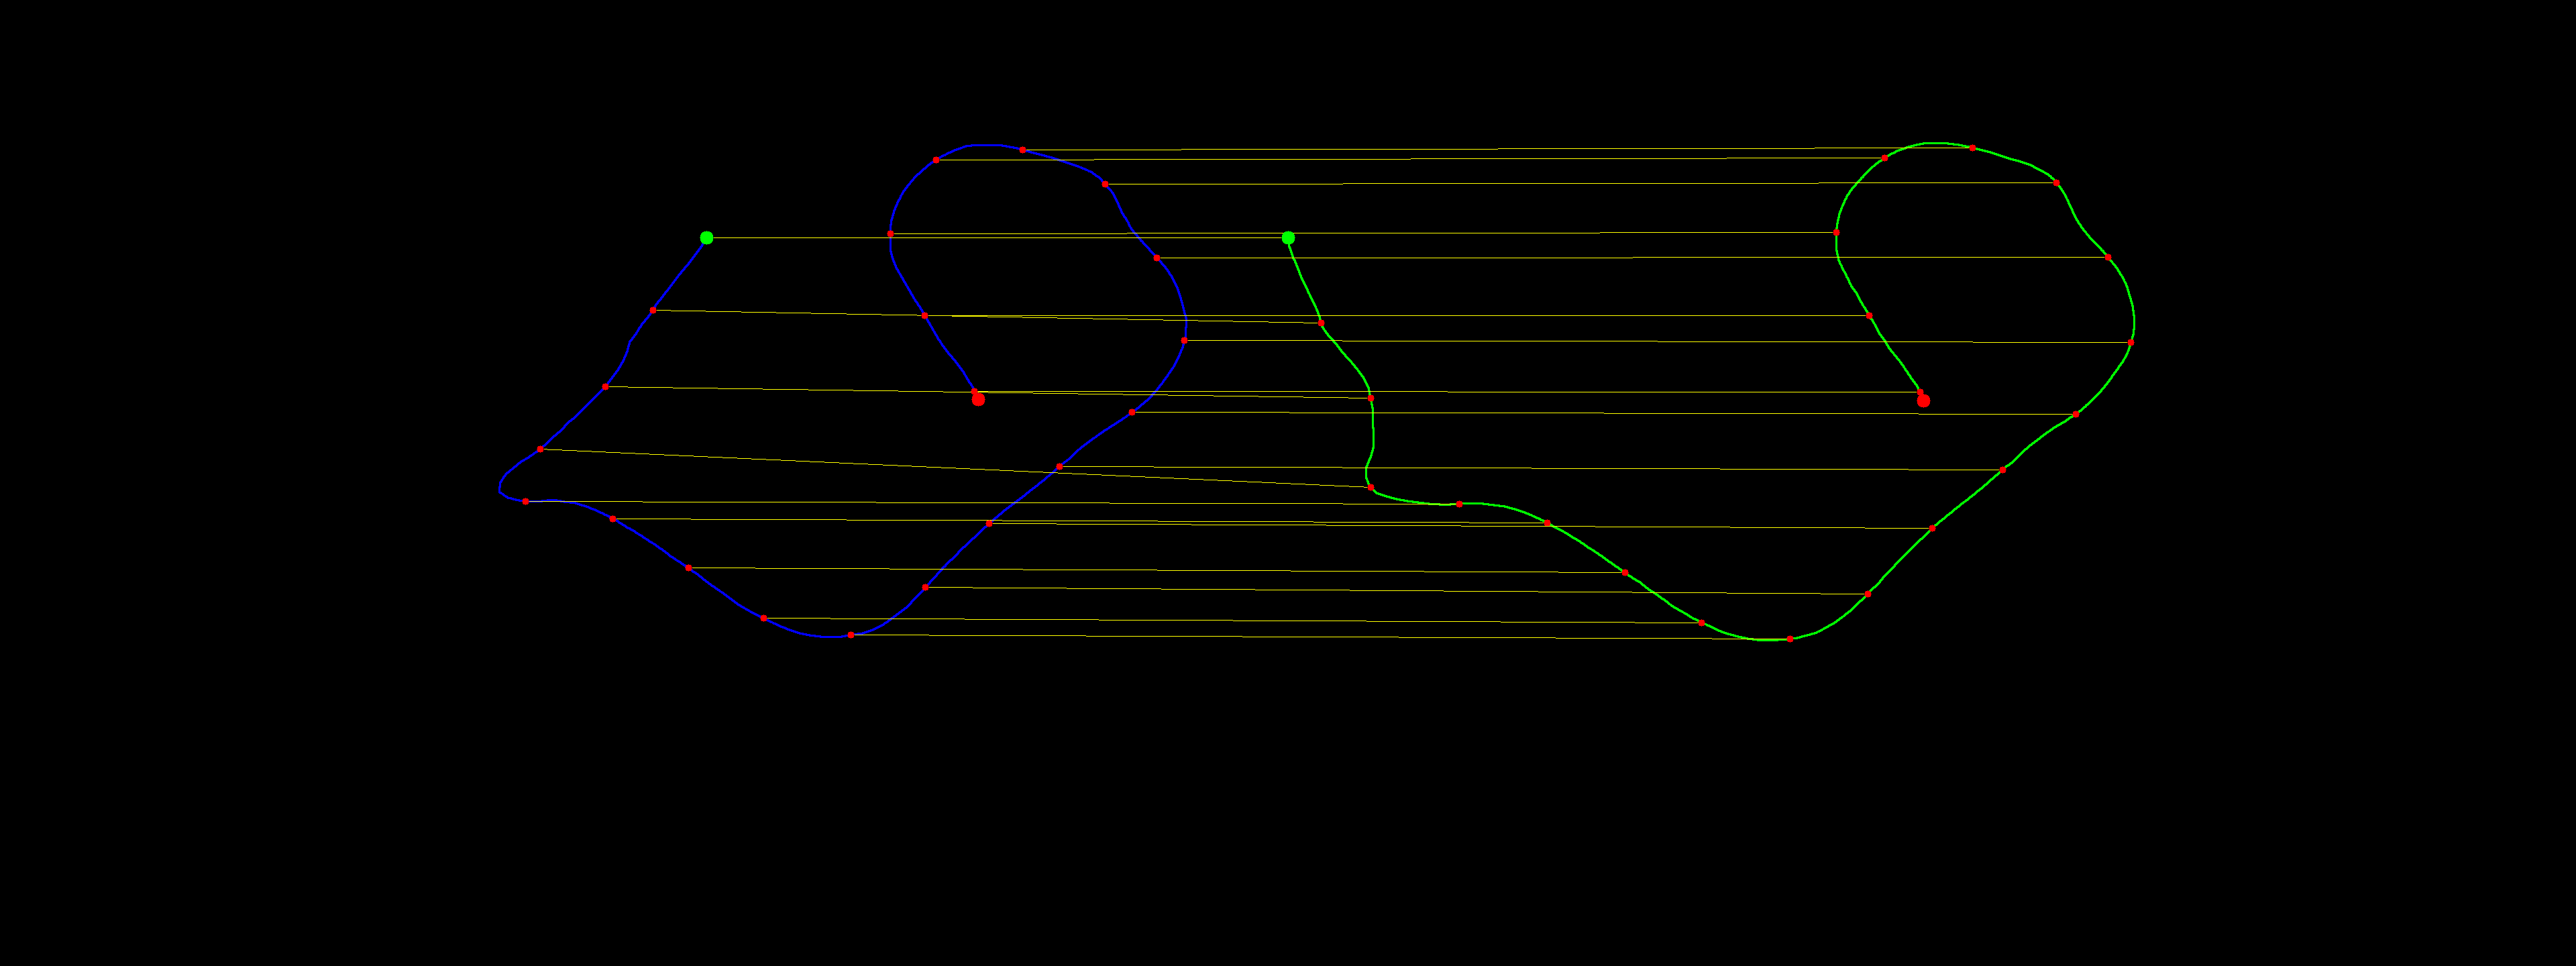
\includegraphics[width=\textwidth]{Images/Figure 6.8.png}
    \caption[Stereo correspondence for Scenario B.]{Stereo correspondence for Scenario B. The noticeably varying lengths of the horizontal matching lines explicitly illustrate the variation in depth along the continuous curve.}
    \label{fig:figure6.8}
\end{figure}

The matched points were triangulated to recover the three-dimensional tether geometry. Figure \ref{fig:figure6.10} presents the final 3D reconstruction obtained for Scenario B. The result demonstrates that the proposed methodology can recover out-of-plane tether deformation and depth variation under low-texture observation conditions.
\newpage
\clearpage

\begin{figure}[!ht]
    \centering
    \begin{minipage}{0.48\textwidth}
        \centering
        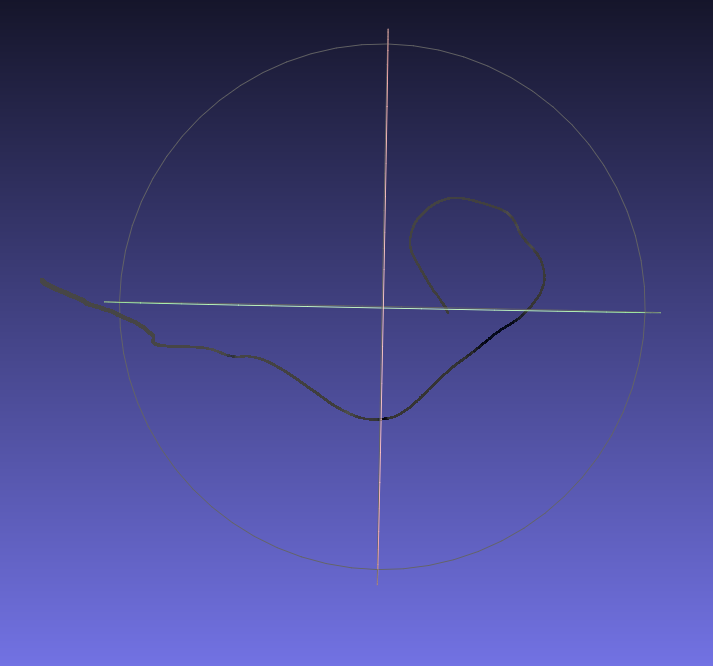
\includegraphics[height=7cm]{Images/Figure 6.10a.png}
    \end{minipage}
    \hfill
    \begin{minipage}{0.48\textwidth}
        \centering
        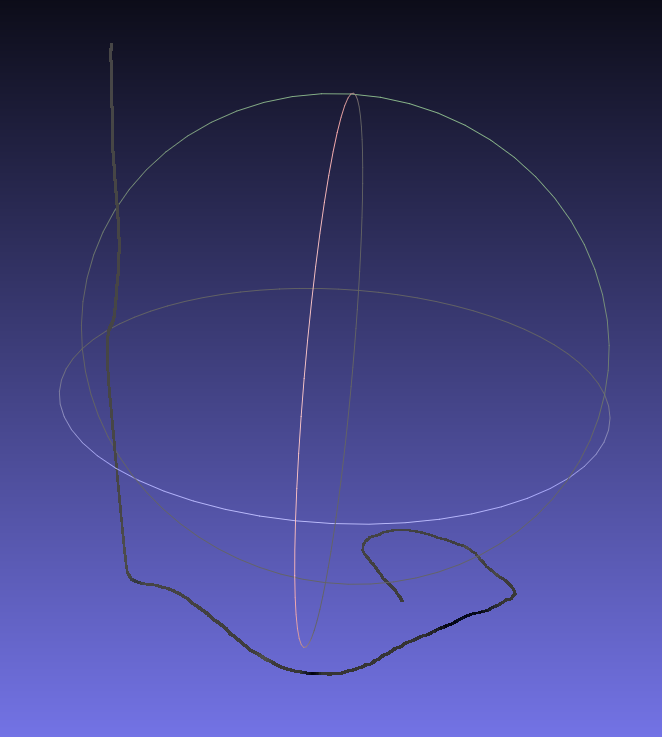
\includegraphics[height=7cm]{Images/Figure 6.10b.png}
    \end{minipage}
    \caption[Final three-dimensional tether reconstruction for scenario B.]{Final three-dimensional tether reconstruction for scenario B. The rotated perspective on the right side explicitly demonstrates the successful recovery of Z-axis depth, confirming the system's capability to monitor complex tether deformations.}
    \label{fig:figure6.10}
\end{figure}

The complete reconstruction sequence for Scenario B is summarized in Figure \ref{fig:figure6.12}, which shows the progression from stereo image acquisition to the final three-dimensional tether representation.

\begin{figure}[!ht]
    \centering
    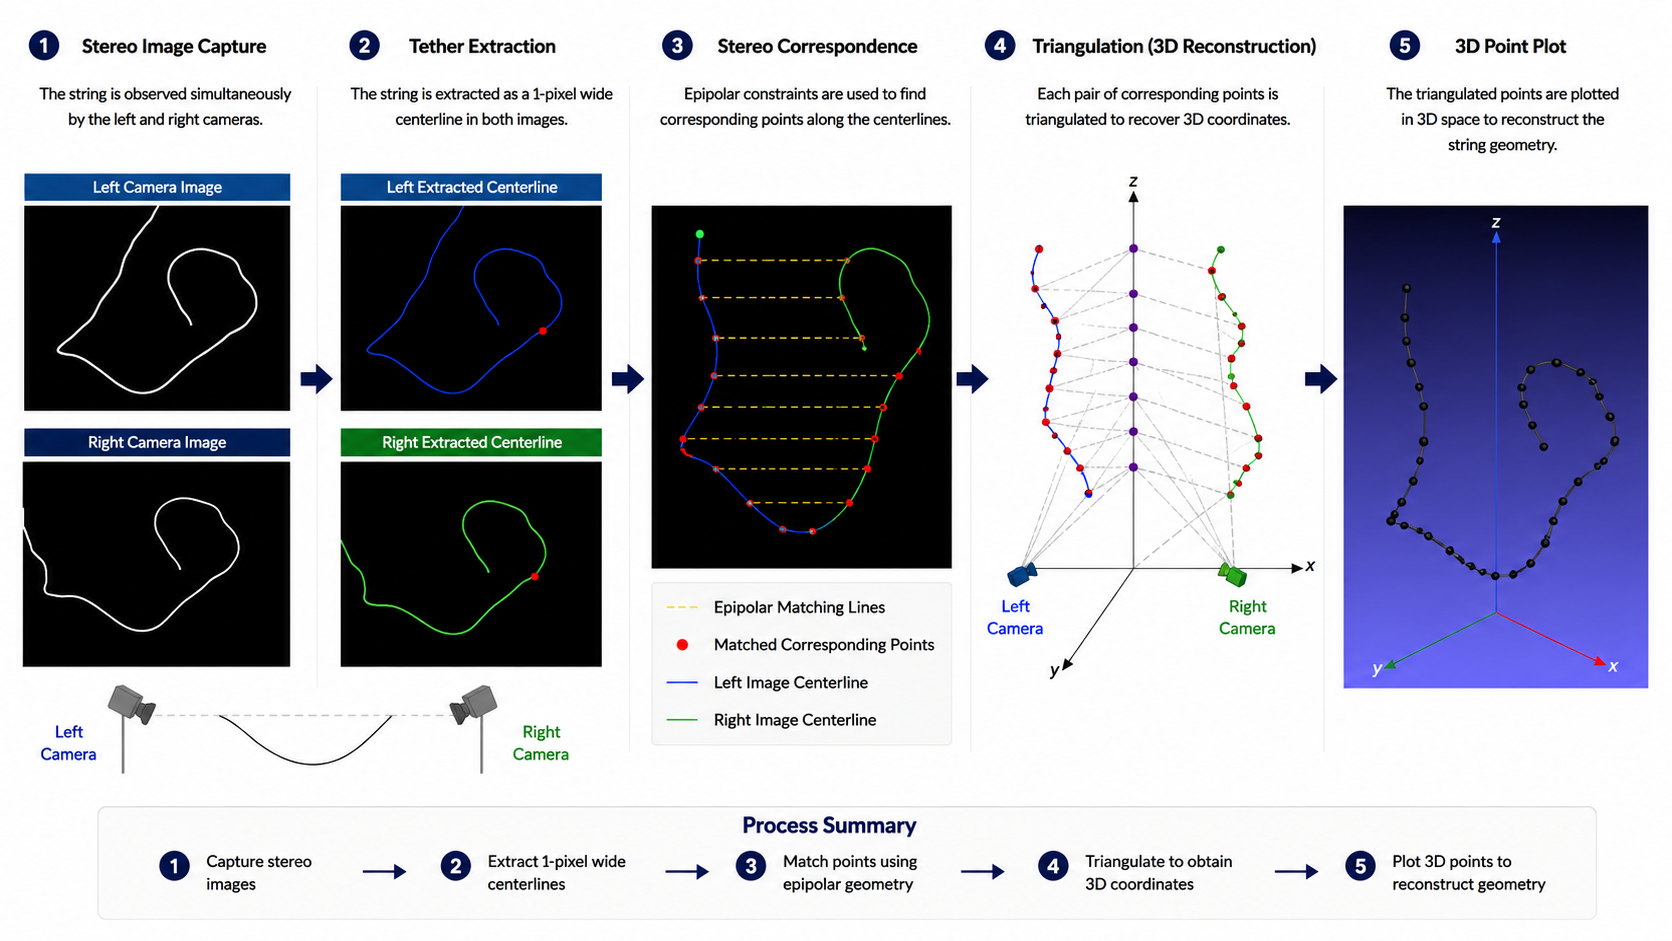
\includegraphics[width=\textwidth]{Images/Figure 6.12.png}
    \caption[Geometry-driven stereo reconstruction workflow from image capture to three-dimensional tether representation in scenario B.]{Geometry-driven Stereo reconstruction workflow from image capture to three-dimensional tether representation in scenario B.}
    \label{fig:figure6.12}
\end{figure}

\subsection{Comparative assessment of scenarios A and B}

The results obtained for both scenarios demonstrate that the geometry-driven reconstruction framework can operate under different tether configurations. Scenario A validated the method under a simpler planar condition, where the stereo disparity remains relatively uniform and the reconstructed tether geometry exhibits limited depth variation.
\\\\
Scenario B provided a more demanding test case, introducing stronger depth variation, perspective effects, and out-of-plane deformation. The successful reconstruction of this configuration demonstrates that the method is not limited to planar tether geometries and can recover more representative three-dimensional shapes.
\\\\
The main difference between both cases is observed in the stereo correspondence stage. Scenario A produced more uniform matching patterns, while Scenario B produced variable correspondence lengths associated with depth changes along the tether. This behavior confirms that the reconstruction pipeline is sensitive to geometric depth variation and can translate stereo disparity differences into three-dimensional tether structure.

\subsection{Topological crossing analysis}

Although the geometry-driven framework successfully reconstructed both tether configurations, complex topological conditions remain an important challenge. In particular, crossings, overlaps, and self-intersections may introduce ambiguity when multiple tether segments project onto nearby or overlapping image regions.
\\\\
The results indicate that these ambiguities do not prevent the reconstruction of the overall tether trajectory, but they can affect local continuity interpretation in highly entangled configurations. This limitation motivates future improvements based on temporal tracking, disparity consistency, and topology-aware processing.
\\\\
These results contrast directly with the failures reported in Section \ref{sec:evaluation-conventional-photogrammetry}. While conventional photogrammetric approaches were unable to reconstruct the tether reliably under low-texture conditions, the geometry-driven methodology produced stable and physically plausible reconstructions for both planar and volumetric tether configurations.

\section{Assessment of AI-assisted reconstruction}

This section does not report an operational reconstruction result; it summarizes an exploratory assessment that was conducted to investigate the potential of AI-based techniques for tether observation. The objective was not to develop an operational reconstruction system but to evaluate whether recent advances in neural reconstruction could inform future versions of the LINKU architecture. This assessment is distinct from the operational segmentation model reported in Section \ref{sec:Geometry-driven stereo reconstruction} and summarized in Figure \ref{fig:ai-status}: this section concerns end-to-end neural \emph{reconstruction} of three-dimensional geometry, which remains exploratory, whereas AI-based \emph{segmentation} has already been implemented and evaluated as a supporting preprocessing step.
\\\\
The assessment focused on the capabilities, limitations, and potential integration pathways of neural methods when applied to thin tether-like structures observed under constrained visual conditions.

\subsection{Evaluation of neural reconstruction methods}

The exploratory investigation considered neural reconstruction approaches capable of inferring three-dimensional geometry from a limited number of images. In particular, Neural Radiance Field (NeRF) methodologies and RealFusion-based reconstruction frameworks were reviewed due to their ability to generate volumetric representations from sparse observations.
\\\\
The assessment confirmed that these methods can infer plausible three-dimensional structures by leveraging geometric priors learned during training. This capability demonstrates the potential of neural approaches to recover information that may be difficult to extract using purely geometric methods.
\\\\
However, the computational requirements of these techniques remain substantially higher than those of the geometry-driven framework developed in this work. Current implementations typically require dedicated GPU acceleration and are not compatible with real-time execution on embedded platforms representative of the proposed flight architecture.

\subsection{Observed limitations}

The exploratory evaluation identified several limitations that currently restrict the use of generative AI models as primary reconstruction tools for scientific tether observation:

\begin{itemize}
    \item Preference for visual plausibility over physical fidelity. Reconstructed outputs often appeared visually coherent but were not always consistent with the actual geometry present in the input observations.
    \item Generation of non-existent features. The models occasionally introduced artificial textures, surface details, or geometric structures that were not present in the original images.
    \item Limited geometric reliability. The reconstructed representations could not guarantee that the inferred shape accurately corresponded to the true three-dimensional tether configuration.
    \item Lack of deterministic behavior. Similar inputs may produce different reconstructions, complicating repeatability and quantitative validation.
    \item Insufficient suitability for scientific measurements. Because reconstruction accuracy is more critical than visual realism for tether monitoring, AI-generated hallucinations represent a significant source of uncertainty.
\end{itemize}

These observations indicate that fully generative reconstruction approaches are not currently suitable as primary sources of scientific tether geometry without additional physical constraints, geometric validation mechanisms, and mission-specific training datasets.

\subsection{Potential roles of AI within LINKU}

Although AI-based reconstruction was not adopted as the primary reconstruction strategy, the assessment identified several areas where neural methods could strengthen the existing geometry-driven framework.
\\\\
One promising application is AI-assisted wire path tracking, which subsumes both ordinary path tracing and topological knot / crossing disambiguation as a single capability rather than two separate ones. As discussed in Section 6.3.4, self-intersections and overlapping tether segments may generate multiple valid interpretations of the observed geometry; a tracker that decides which branch to follow at each ambiguous point is solving exactly the same problem whether the thread is mostly straight (few or no ambiguous points) or heavily entangled (many of them). Section \ref{sec:Geometry-driven stereo reconstruction} (Figure \ref{fig:ai-proposed-tracker}) proposes a concrete design for this component, built by replacing the fixed, hand-tuned decision rule inside the already-implemented tracker with a learned one.
\\\\
A second opportunity is tether segmentation, where a first implementation already exists: a pixel-level Random Forest classifier, described in Section \ref{sec:Geometry-driven stereo reconstruction}, is currently used as a selectable alternative to manual threshold tuning. Lightweight neural architectures, such as U-Net-based models, represent a natural next iteration of this same component and could further improve mask generation under challenging illumination conditions, including specular reflections and high-contrast observations.
\\\\
These results suggest that the most effective role of AI within LINKU is as a supporting technology for perception and ambiguity resolution, while geometric reconstruction remains the responsibility of the physics-based stereo pipeline.

\section{Comparative discussion}

The experimental investigation evaluated three distinct approaches for tether reconstruction under space-emulated observation conditions: conventional photogrammetry, geometry-driven stereo reconstruction, and AI-assisted reconstruction. Each approach exhibited different capabilities, limitations, and operational requirements.
\\\\
To facilitate comparison, this section walks through both pipelines stage by stage, starting from the same stereo capture, and states exactly where each one succeeds or fails under the experimental conditions investigated in this work, rather than summarizing them as qualitative criterion-by-criterion ratings.

\subsection{Conventional photogrammetry vs geometry-driven reconstruction}

Both pipelines start from the same input: a synchronized stereo image pair. From that point, they diverge immediately.
\\\\
Conventional photogrammetry proceeds as feature detection (keypoints) $\rightarrow$ feature matching $\rightarrow$ triangulation. This pipeline breaks at the very first stage: a tether that occupies only 1--3 pixels does not provide enough distinctive keypoints for reliable detection, so feature matching and triangulation never receive usable input. This limitation persisted even after the tether was perfectly isolated from all background texture, producing the ``Zero Resolution'' failure reported in Section \ref{sub:tether-reconstruction-failure} (Figure \ref{fig:figure6.4}). Acceptable performance can still be achieved for volumetric objects with abundant texture under favorable imaging conditions, but the approach fails as soon as it is applied to a thin structure against a featureless background.
\\\\
The geometry-driven pipeline proceeds instead as intensity extraction and segmentation $\rightarrow$ skeleton and endpoint detection $\rightarrow$ curve tracking (Figure \ref{fig:pipeline-implementation}) $\rightarrow$ stereo correspondence via normalized cross-correlation along the epipolar line $\rightarrow$ triangulation. None of these stages require keypoints: radiometric contrast and geometric continuity are sufficient on their own. This is precisely why the pipeline succeeds where the conventional one fails, and it produced stable reconstructions for both the planar and volumetric tether configurations (Figures \ref{fig:figure6.9} and \ref{fig:figure6.10}).
\newpage
\clearpage

\subsection{Geometry-driven vs AI-assisted reconstruction}

Unlike the comparison above, geometry-driven reconstruction and AI-assisted wire path tracking are not two competing pipelines evaluated side by side experimentally -- only the former has been implemented and tested. The comparison here is therefore architectural: Figure \ref{fig:ai-proposed-tracker} (Section \ref{sec:Geometry-driven stereo reconstruction}) shows that the proposed AI component does not replace the geometry-driven search; it reuses the exact same step-by-step tracker already implemented and validated in this chapter, and only swaps the fixed, hand-tuned branch-scoring rule for a learned one trained on operator-verified paths.
\\\\
This has two direct consequences for how the two approaches compare. First, every property that makes the geometry-driven framework attractive for a scientific mission -- a deterministic search, physically grounded features (direction, thickness, centeredness), and traceable intermediate results -- is preserved in the proposed AI variant, because the search itself is not learned, only the local scoring weights are. Second, the risk categories usually associated with generative AI reconstruction (hallucinated geometry, non-deterministic outputs, lack of physical grounding) apply to the end-to-end neural methods assessed in Section \ref{sec:evaluation-conventional-photogrammetry} (NeRF, RealFusion), not to this proposed component: a mis-scored branch produces a locally wrong path segment that remains subject to the same backtracking and downstream consistency checks as the classical tracker, rather than an unconstrained hallucinated shape.
\\\\
The geometry-driven framework provides physically interpretable and repeatable reconstructions directly linked to the observed image measurements. This characteristic is particularly important for scientific missions, where reconstruction fidelity and traceability are more critical than visual realism. The exploratory AI assessment revealed promising capabilities in perception-oriented tasks, particularly for segmentation (already implemented, Figure \ref{fig:ai-status}) and, prospectively, for path tracking through topologically ambiguous configurations. However, the tendency of fully generative models to introduce non-physical structures limits their suitability as primary reconstruction engines. Consequently, AI is currently better positioned as a complementary technology that enhances specific, well-bounded stages of the reconstruction pipeline rather than replacing the underlying geometric framework.

\subsection{Implications for future tether observation missions}

The results obtained throughout this chapter indicate that future tether observation systems should prioritize physics-based geometric reconstruction as the primary source of scientific measurements. Conventional photogrammetric methods were shown to be inadequate for thin, low-texture structures, while the proposed geometry-driven framework successfully recovered tether geometry under both planar and volumetric configurations.
\\\\
The exploratory assessment of AI-based techniques further suggests that neural methods are most valuable when applied to perception and ambiguity-resolution tasks rather than direct geometric reconstruction. In particular, future developments may benefit from AI-assisted wire path tracking -- covering both ordinary tracing and topological knot/crossing resolution as one capability -- and from further iterations of the already-implemented segmentation model to improve robustness under challenging illumination conditions.
\\\\
These findings support a hybrid architecture in which geometric reconstruction provides physically interpretable measurements, while AI modules enhance robustness in specific operational scenarios. Such an approach offers a practical path toward reliable tether monitoring systems for future orbital deployment and inspection missions.

